\documentclass[twoside]{book}

% Packages required by doxygen
\usepackage{calc}
\usepackage{doxygen}
\usepackage{graphicx}
\usepackage[utf8]{inputenc}
\usepackage{makeidx}
\usepackage{multicol}
\usepackage{multirow}
\usepackage{textcomp}
\usepackage[table]{xcolor}

% Font selection
\usepackage[T1]{fontenc}
\usepackage{mathptmx}
\usepackage[scaled=.90]{helvet}
\usepackage{courier}
\usepackage{amssymb}
\usepackage{sectsty}
\renewcommand{\familydefault}{\sfdefault}
\allsectionsfont{%
  \fontseries{bc}\selectfont%
  \color{darkgray}%
}
\renewcommand{\DoxyLabelFont}{%
  \fontseries{bc}\selectfont%
  \color{darkgray}%
}

% Page & text layout
\usepackage{geometry}
\geometry{%
  a4paper,%
  top=2.5cm,%
  bottom=2.5cm,%
  left=2.5cm,%
  right=2.5cm%
}
\tolerance=750
\hfuzz=15pt
\hbadness=750
\setlength{\emergencystretch}{15pt}
\setlength{\parindent}{0cm}
\setlength{\parskip}{0.2cm}
\makeatletter
\renewcommand{\paragraph}{%
  \@startsection{paragraph}{4}{0ex}{-1.0ex}{1.0ex}{%
    \normalfont\normalsize\bfseries\SS@parafont%
  }%
}
\renewcommand{\subparagraph}{%
  \@startsection{subparagraph}{5}{0ex}{-1.0ex}{1.0ex}{%
    \normalfont\normalsize\bfseries\SS@subparafont%
  }%
}
\makeatother

% Headers & footers
\usepackage{fancyhdr}
\pagestyle{fancyplain}
\fancyhead[LE]{\fancyplain{}{\bfseries\thepage}}
\fancyhead[CE]{\fancyplain{}{}}
\fancyhead[RE]{\fancyplain{}{\bfseries\leftmark}}
\fancyhead[LO]{\fancyplain{}{\bfseries\rightmark}}
\fancyhead[CO]{\fancyplain{}{}}
\fancyhead[RO]{\fancyplain{}{\bfseries\thepage}}
\fancyfoot[LE]{\fancyplain{}{}}
\fancyfoot[CE]{\fancyplain{}{}}
\fancyfoot[RE]{\fancyplain{}{\bfseries\scriptsize Generated on Mon Feb 3 2014 14\-:56\-:13 for Avaliação de Formações com Dados de Teste de Pressão by Doxygen }}
\fancyfoot[LO]{\fancyplain{}{\bfseries\scriptsize Generated on Mon Feb 3 2014 14\-:56\-:13 for Avaliação de Formações com Dados de Teste de Pressão by Doxygen }}
\fancyfoot[CO]{\fancyplain{}{}}
\fancyfoot[RO]{\fancyplain{}{}}
\renewcommand{\footrulewidth}{0.4pt}
\renewcommand{\chaptermark}[1]{%
  \markboth{#1}{}%
}
\renewcommand{\sectionmark}[1]{%
  \markright{\thesection\ #1}%
}

% Indices & bibliography
\usepackage{natbib}
\usepackage[titles]{tocloft}
\setcounter{tocdepth}{3}
\setcounter{secnumdepth}{5}
\makeindex

% Hyperlinks (required, but should be loaded last)
\usepackage{ifpdf}
\ifpdf
  \usepackage[pdftex,pagebackref=true]{hyperref}
\else
  \usepackage[ps2pdf,pagebackref=true]{hyperref}
\fi
\hypersetup{%
  colorlinks=true,%
  linkcolor=blue,%
  citecolor=blue,%
  unicode%
}

% Custom commands
\newcommand{\clearemptydoublepage}{%
  \newpage{\pagestyle{empty}\cleardoublepage}%
}


%===== C O N T E N T S =====

\begin{document}

% Titlepage & ToC
\hypersetup{pageanchor=false}
\pagenumbering{roman}
\begin{titlepage}
\vspace*{7cm}
\begin{center}%
{\Large Avaliação de Formações com Dados de Teste de Pressão }\\
\vspace*{1cm}
{\large Generated by Doxygen 1.8.6}\\
\vspace*{0.5cm}
{\small Mon Feb 3 2014 14:56:13}\\
\end{center}
\end{titlepage}
\clearemptydoublepage
\tableofcontents
\clearemptydoublepage
\pagenumbering{arabic}
\hypersetup{pageanchor=true}

%--- Begin generated contents ---
\chapter{Hierarchical Index}
\section{Class Hierarchy}
This inheritance list is sorted roughly, but not completely, alphabetically\-:\begin{DoxyCompactList}
\item \contentsline{section}{C\-Ajuste\-Curva\-Minimos\-Quadrados}{\pageref{classCAjusteCurvaMinimosQuadrados}}{}
\begin{DoxyCompactList}
\item \contentsline{section}{C\-Ajuste\-Curva}{\pageref{classCAjusteCurva}}{}
\end{DoxyCompactList}
\item \contentsline{section}{C\-Caracterizacao\-Reservatorio}{\pageref{classCCaracterizacaoReservatorio}}{}
\item \contentsline{section}{C\-Dados\-Registrador\-Pressao}{\pageref{classCDadosRegistradorPressao}}{}
\item \contentsline{section}{C\-Estatistica}{\pageref{classCEstatistica}}{}
\item \contentsline{section}{C\-Fluido}{\pageref{classCFluido}}{}
\item \contentsline{section}{C\-Poco}{\pageref{classCPoco}}{}
\item \contentsline{section}{C\-Reservatorio}{\pageref{classCReservatorio}}{}
\item \contentsline{section}{C\-Simulador\-Analise\-Teste\-Pressao}{\pageref{classCSimuladorAnaliseTestePressao}}{}
\item \contentsline{section}{Gnuplot}{\pageref{classGnuplot}}{}
\item runtime\-\_\-error\begin{DoxyCompactList}
\item \contentsline{section}{Gnuplot\-Exception}{\pageref{classGnuplotException}}{}
\end{DoxyCompactList}
\end{DoxyCompactList}

\chapter{Class Index}
\section{Class List}
Here are the classes, structs, unions and interfaces with brief descriptions\-:\begin{DoxyCompactList}
\item\contentsline{section}{\hyperlink{classCAjusteCurva}{C\-Ajuste\-Curva} \\*Classe que executa a regressao linear e ajusta ate a correlacao satisfatoria }{\pageref{classCAjusteCurva}}{}
\item\contentsline{section}{\hyperlink{classCAjusteCurvaMinimosQuadrados}{C\-Ajuste\-Curva\-Minimos\-Quadrados} \\*Classe que obtem os coeficiente da regressao linear por meio do metodo dos minimos quadrados }{\pageref{classCAjusteCurvaMinimosQuadrados}}{}
\item\contentsline{section}{\hyperlink{classCCaracterizacaoReservatorio}{C\-Caracterizacao\-Reservatorio} \\*Classe que caracteriza o reservatorio }{\pageref{classCCaracterizacaoReservatorio}}{}
\item\contentsline{section}{\hyperlink{classCDadosRegistradorPressao}{C\-Dados\-Registrador\-Pressao} \\*Classe que contem dados registrados do registrador de pressao }{\pageref{classCDadosRegistradorPressao}}{}
\item\contentsline{section}{\hyperlink{classCEstatistica}{C\-Estatistica} \\*Classe que calcula estatisticas do vetor, como media e desvio padrao, util para regressao }{\pageref{classCEstatistica}}{}
\item\contentsline{section}{\hyperlink{classCFluido}{C\-Fluido} \\*Classe contendo as caracteristicas do fluido produzido }{\pageref{classCFluido}}{}
\item\contentsline{section}{\hyperlink{classCPoco}{C\-Poco} \\*Classe contendo as caracteristicas do poco }{\pageref{classCPoco}}{}
\item\contentsline{section}{\hyperlink{classCReservatorio}{C\-Reservatorio} \\*Classe contendo as caracteristicas do reservatorio }{\pageref{classCReservatorio}}{}
\item\contentsline{section}{\hyperlink{classCSimuladorAnaliseTestePressao}{C\-Simulador\-Analise\-Teste\-Pressao} \\*Classe que faz a analise do teste de pressao realizado no campo e infere as propriedades do reservatorio }{\pageref{classCSimuladorAnaliseTestePressao}}{}
\item\contentsline{section}{\hyperlink{classGnuplot}{Gnuplot} \\*Classe de interface para acesso ao programa gnuplot }{\pageref{classGnuplot}}{}
\item\contentsline{section}{\hyperlink{classGnuplotException}{Gnuplot\-Exception} \\*Erros em tempo de execucao }{\pageref{classGnuplotException}}{}
\end{DoxyCompactList}

\chapter{Class Documentation}
\hypertarget{classCAjusteCurva}{\section{C\-Ajuste\-Curva Class Reference}
\label{classCAjusteCurva}\index{C\-Ajuste\-Curva@{C\-Ajuste\-Curva}}
}


Classe que executa a regressao linear e ajusta ate a correlacao satisfatoria.  




{\ttfamily \#include $<$C\-Ajuste\-Curva.\-h$>$}



Inheritance diagram for C\-Ajuste\-Curva\-:
\nopagebreak
\begin{figure}[H]
\begin{center}
\leavevmode
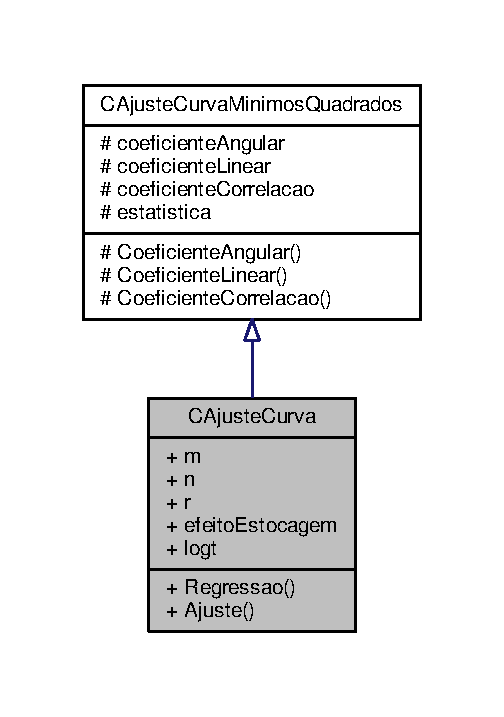
\includegraphics[width=242pt]{classCAjusteCurva__inherit__graph}
\end{center}
\end{figure}


Collaboration diagram for C\-Ajuste\-Curva\-:
\nopagebreak
\begin{figure}[H]
\begin{center}
\leavevmode
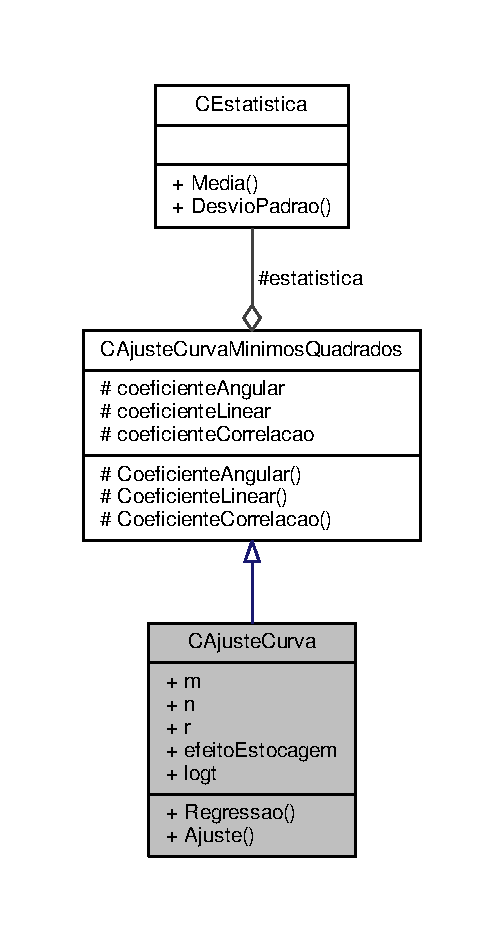
\includegraphics[width=242pt]{classCAjusteCurva__coll__graph}
\end{center}
\end{figure}
\subsection*{Public Member Functions}
\begin{DoxyCompactItemize}
\item 
\hypertarget{classCAjusteCurva_a0687a76e2f668770408276cf0b9731a5}{void \hyperlink{classCAjusteCurva_a0687a76e2f668770408276cf0b9731a5}{Regressao} (std\-::vector$<$ double $>$ vx, std\-::vector$<$ double $>$ vy, double z)}\label{classCAjusteCurva_a0687a76e2f668770408276cf0b9731a5}

\begin{DoxyCompactList}\small\item\em Funcao que executa a regressao linear atraves do metodo dos minimos quadrados. \end{DoxyCompactList}\item 
\hypertarget{classCAjusteCurva_aa7a0c356cb514926d8fcc96f069744b3}{void \hyperlink{classCAjusteCurva_aa7a0c356cb514926d8fcc96f069744b3}{Ajuste} (std\-::vector$<$ double $>$ vx, std\-::vector$<$ double $>$ vy, double z)}\label{classCAjusteCurva_aa7a0c356cb514926d8fcc96f069744b3}

\begin{DoxyCompactList}\small\item\em Funcao que ajusta a regressao para o periodo correto, removendo os pontos referentes a estocagem. \end{DoxyCompactList}\end{DoxyCompactItemize}
\subsection*{Public Attributes}
\begin{DoxyCompactItemize}
\item 
\hypertarget{classCAjusteCurva_ad475e0f4f3c7b77bf10a00e4adb46282}{double \hyperlink{classCAjusteCurva_ad475e0f4f3c7b77bf10a00e4adb46282}{m}}\label{classCAjusteCurva_ad475e0f4f3c7b77bf10a00e4adb46282}

\begin{DoxyCompactList}\small\item\em coef. angular \end{DoxyCompactList}\item 
\hypertarget{classCAjusteCurva_a5c75119dc972a7c7cfd067a9b74c3642}{double \hyperlink{classCAjusteCurva_a5c75119dc972a7c7cfd067a9b74c3642}{n}}\label{classCAjusteCurva_a5c75119dc972a7c7cfd067a9b74c3642}

\begin{DoxyCompactList}\small\item\em coef. linear \end{DoxyCompactList}\item 
\hypertarget{classCAjusteCurva_a21ca23b4c39833776028822f3de6758b}{double \hyperlink{classCAjusteCurva_a21ca23b4c39833776028822f3de6758b}{r}}\label{classCAjusteCurva_a21ca23b4c39833776028822f3de6758b}

\begin{DoxyCompactList}\small\item\em coef. de correlacao \end{DoxyCompactList}\item 
\hypertarget{classCAjusteCurva_a193c50c4214e29b8ed43d6023d42e47a}{bool \hyperlink{classCAjusteCurva_a193c50c4214e29b8ed43d6023d42e47a}{efeito\-Estocagem}}\label{classCAjusteCurva_a193c50c4214e29b8ed43d6023d42e47a}

\begin{DoxyCompactList}\small\item\em indica que o coef. de correlacao nao foi satisfatorio (ha estocagem) \end{DoxyCompactList}\item 
\hypertarget{classCAjusteCurva_a98acb361b2bfb83752d043d0cd0e7e6e}{std\-::vector$<$ double $>$ \hyperlink{classCAjusteCurva_a98acb361b2bfb83752d043d0cd0e7e6e}{logt}}\label{classCAjusteCurva_a98acb361b2bfb83752d043d0cd0e7e6e}

\begin{DoxyCompactList}\small\item\em ajuste de variavel para logaritmica \end{DoxyCompactList}\end{DoxyCompactItemize}
\subsection*{Additional Inherited Members}


\subsection{Detailed Description}
Classe que executa a regressao linear e ajusta ate a correlacao satisfatoria. 

The documentation for this class was generated from the following files\-:\begin{DoxyCompactItemize}
\item 
C\-Ajuste\-Curva.\-h\item 
C\-Ajuste\-Curva.\-cpp\end{DoxyCompactItemize}

\hypertarget{classCAjusteCurvaMinimosQuadrados}{\section{C\-Ajuste\-Curva\-Minimos\-Quadrados Class Reference}
\label{classCAjusteCurvaMinimosQuadrados}\index{C\-Ajuste\-Curva\-Minimos\-Quadrados@{C\-Ajuste\-Curva\-Minimos\-Quadrados}}
}


Classe que obtem os coeficiente da regressao linear por meio do metodo dos minimos quadrados.  




{\ttfamily \#include $<$C\-Ajuste\-Curva\-Minimos\-Quadrados.\-h$>$}



Inheritance diagram for C\-Ajuste\-Curva\-Minimos\-Quadrados\-:
\nopagebreak
\begin{figure}[H]
\begin{center}
\leavevmode
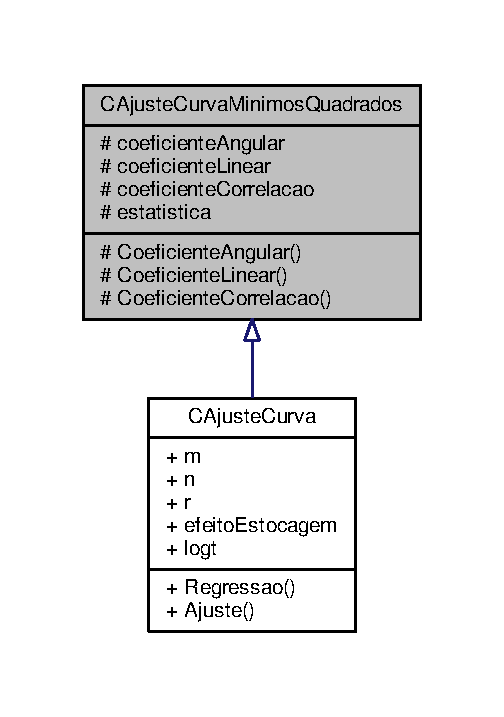
\includegraphics[width=242pt]{classCAjusteCurvaMinimosQuadrados__inherit__graph}
\end{center}
\end{figure}


Collaboration diagram for C\-Ajuste\-Curva\-Minimos\-Quadrados\-:
\nopagebreak
\begin{figure}[H]
\begin{center}
\leavevmode
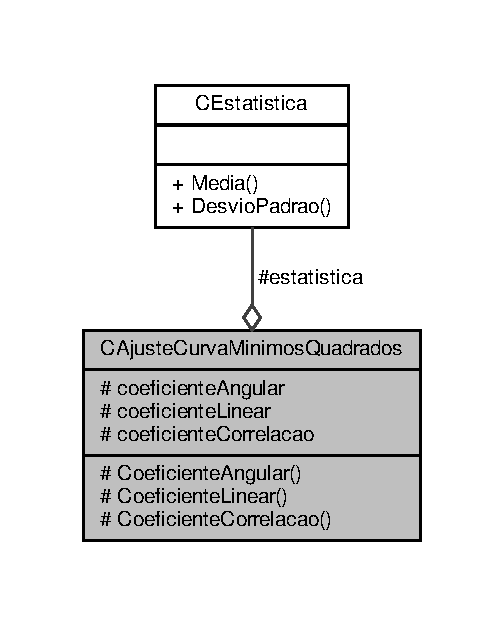
\includegraphics[width=242pt]{classCAjusteCurvaMinimosQuadrados__coll__graph}
\end{center}
\end{figure}
\subsection*{Protected Member Functions}
\begin{DoxyCompactItemize}
\item 
\hypertarget{classCAjusteCurvaMinimosQuadrados_a19b822bde587b27923e67607f3a19c5b}{double \hyperlink{classCAjusteCurvaMinimosQuadrados_a19b822bde587b27923e67607f3a19c5b}{Coeficiente\-Angular} (std\-::vector$<$ double $>$ vx, std\-::vector$<$ double $>$ vy)}\label{classCAjusteCurvaMinimosQuadrados_a19b822bde587b27923e67607f3a19c5b}

\begin{DoxyCompactList}\small\item\em Funcao que retorna o valor do coeficiente angular. \end{DoxyCompactList}\item 
\hypertarget{classCAjusteCurvaMinimosQuadrados_a6f59fda309b84961724af2c065bff236}{double \hyperlink{classCAjusteCurvaMinimosQuadrados_a6f59fda309b84961724af2c065bff236}{Coeficiente\-Linear} (std\-::vector$<$ double $>$ vx, std\-::vector$<$ double $>$ vy)}\label{classCAjusteCurvaMinimosQuadrados_a6f59fda309b84961724af2c065bff236}

\begin{DoxyCompactList}\small\item\em Funcao que retorna o valor do coeficiente linear. \end{DoxyCompactList}\item 
\hypertarget{classCAjusteCurvaMinimosQuadrados_a5900f85b41ce140613d1ac31077549c5}{double \hyperlink{classCAjusteCurvaMinimosQuadrados_a5900f85b41ce140613d1ac31077549c5}{Coeficiente\-Correlacao} (std\-::vector$<$ double $>$ vx, std\-::vector$<$ double $>$ vy)}\label{classCAjusteCurvaMinimosQuadrados_a5900f85b41ce140613d1ac31077549c5}

\begin{DoxyCompactList}\small\item\em Funcao que retorna o valor do coeficiente de correlacao. \end{DoxyCompactList}\end{DoxyCompactItemize}
\subsection*{Protected Attributes}
\begin{DoxyCompactItemize}
\item 
\hypertarget{classCAjusteCurvaMinimosQuadrados_a9acb25b94e4197b4438354a3cc0149d8}{double \hyperlink{classCAjusteCurvaMinimosQuadrados_a9acb25b94e4197b4438354a3cc0149d8}{coeficiente\-Angular}}\label{classCAjusteCurvaMinimosQuadrados_a9acb25b94e4197b4438354a3cc0149d8}

\begin{DoxyCompactList}\small\item\em coeficiente angular da reta do tipo y=ax+b \end{DoxyCompactList}\item 
\hypertarget{classCAjusteCurvaMinimosQuadrados_a773d82a76e8328f285dad4d1272cad53}{double \hyperlink{classCAjusteCurvaMinimosQuadrados_a773d82a76e8328f285dad4d1272cad53}{coeficiente\-Linear}}\label{classCAjusteCurvaMinimosQuadrados_a773d82a76e8328f285dad4d1272cad53}

\begin{DoxyCompactList}\small\item\em coeficiente linear da reta do tipo y=ax+b \end{DoxyCompactList}\item 
\hypertarget{classCAjusteCurvaMinimosQuadrados_acdac37bfab1829fa6594244b725b21be}{double \hyperlink{classCAjusteCurvaMinimosQuadrados_acdac37bfab1829fa6594244b725b21be}{coeficiente\-Correlacao}}\label{classCAjusteCurvaMinimosQuadrados_acdac37bfab1829fa6594244b725b21be}

\begin{DoxyCompactList}\small\item\em coeficiente de correlacao da reta do tipo y=ax+b \end{DoxyCompactList}\item 
\hypertarget{classCAjusteCurvaMinimosQuadrados_a5d05f026e862a7864a506fd44dda2a07}{\hyperlink{classCEstatistica}{C\-Estatistica} \hyperlink{classCAjusteCurvaMinimosQuadrados_a5d05f026e862a7864a506fd44dda2a07}{estatistica}}\label{classCAjusteCurvaMinimosQuadrados_a5d05f026e862a7864a506fd44dda2a07}

\begin{DoxyCompactList}\small\item\em cria um objeto da classe \hyperlink{classCEstatistica}{C\-Estatistica} para ser utilizado funcoes de calculo \end{DoxyCompactList}\end{DoxyCompactItemize}


\subsection{Detailed Description}
Classe que obtem os coeficiente da regressao linear por meio do metodo dos minimos quadrados. 

The documentation for this class was generated from the following files\-:\begin{DoxyCompactItemize}
\item 
C\-Ajuste\-Curva\-Minimos\-Quadrados.\-h\item 
C\-Ajuste\-Curva\-Minimos\-Quadrados.\-cpp\end{DoxyCompactItemize}

\hypertarget{classCCaracterizacaoReservatorio}{\section{C\-Caracterizacao\-Reservatorio Class Reference}
\label{classCCaracterizacaoReservatorio}\index{C\-Caracterizacao\-Reservatorio@{C\-Caracterizacao\-Reservatorio}}
}


Classe que caracteriza o reservatorio.  




{\ttfamily \#include $<$C\-Caracterizacao\-Reservatorio.\-h$>$}



Collaboration diagram for C\-Caracterizacao\-Reservatorio\-:
\nopagebreak
\begin{figure}[H]
\begin{center}
\leavevmode
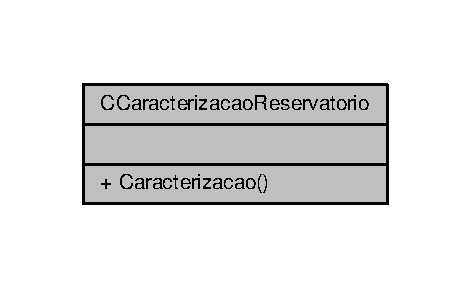
\includegraphics[width=226pt]{classCCaracterizacaoReservatorio__coll__graph}
\end{center}
\end{figure}
\subsection*{Public Member Functions}
\begin{DoxyCompactItemize}
\item 
\hypertarget{classCCaracterizacaoReservatorio_af1a321279cc36b716acdf44aab4905da}{void \hyperlink{classCCaracterizacaoReservatorio_af1a321279cc36b716acdf44aab4905da}{Caracterizacao} (double permeabilidade, double fatorpelicula, double indiceprodutividade, double raiopoco, double raioefetivo)}\label{classCCaracterizacaoReservatorio_af1a321279cc36b716acdf44aab4905da}

\begin{DoxyCompactList}\small\item\em Funcao que analisa os resultados e caracteriza o reservatorio. \end{DoxyCompactList}\end{DoxyCompactItemize}


\subsection{Detailed Description}
Classe que caracteriza o reservatorio. 

The documentation for this class was generated from the following files\-:\begin{DoxyCompactItemize}
\item 
C\-Caracterizacao\-Reservatorio.\-h\item 
C\-Caracterizacao\-Reservatorio.\-cpp\end{DoxyCompactItemize}

\hypertarget{classCDadosRegistradorPressao}{\section{C\-Dados\-Registrador\-Pressao Class Reference}
\label{classCDadosRegistradorPressao}\index{C\-Dados\-Registrador\-Pressao@{C\-Dados\-Registrador\-Pressao}}
}


Classe que contem dados registrados do registrador de pressao.  




{\ttfamily \#include $<$C\-Dados\-Registrador\-Pressao.\-h$>$}



Collaboration diagram for C\-Dados\-Registrador\-Pressao\-:
\nopagebreak
\begin{figure}[H]
\begin{center}
\leavevmode
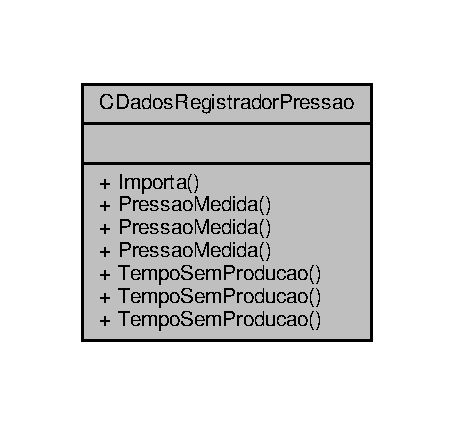
\includegraphics[width=218pt]{classCDadosRegistradorPressao__coll__graph}
\end{center}
\end{figure}
\subsection*{Public Member Functions}
\begin{DoxyCompactItemize}
\item 
\hypertarget{classCDadosRegistradorPressao_af0d2c2b61c6300ff81918e294e19deb9}{void \hyperlink{classCDadosRegistradorPressao_af0d2c2b61c6300ff81918e294e19deb9}{Importa} ()}\label{classCDadosRegistradorPressao_af0d2c2b61c6300ff81918e294e19deb9}

\begin{DoxyCompactList}\small\item\em Funcao que importa os dados registrados do arquivo .dat, preenchendo os atributos da classe. \end{DoxyCompactList}\item 
\hypertarget{classCDadosRegistradorPressao_a3c044f2142c298c11d56a375979ff5fd}{void \hyperlink{classCDadosRegistradorPressao_a3c044f2142c298c11d56a375979ff5fd}{Pressao\-Medida} (std\-::vector$<$ double $>$ \-\_\-pressao\-Medida)}\label{classCDadosRegistradorPressao_a3c044f2142c298c11d56a375979ff5fd}

\begin{DoxyCompactList}\small\item\em Funcao que seta a pressaomedida. \end{DoxyCompactList}\item 
\hypertarget{classCDadosRegistradorPressao_adacef1440655206361ba87c6b0fd7b8c}{double \hyperlink{classCDadosRegistradorPressao_adacef1440655206361ba87c6b0fd7b8c}{Pressao\-Medida} (int posicao) const }\label{classCDadosRegistradorPressao_adacef1440655206361ba87c6b0fd7b8c}

\begin{DoxyCompactList}\small\item\em Funcao get da posicao informada do vetor pressaomedida. \end{DoxyCompactList}\item 
\hypertarget{classCDadosRegistradorPressao_a647d831edf3669d97b239484bede72ec}{std\-::vector$<$ double $>$ \hyperlink{classCDadosRegistradorPressao_a647d831edf3669d97b239484bede72ec}{Pressao\-Medida} () const }\label{classCDadosRegistradorPressao_a647d831edf3669d97b239484bede72ec}

\begin{DoxyCompactList}\small\item\em Funcao get da pressaomedida. \end{DoxyCompactList}\item 
\hypertarget{classCDadosRegistradorPressao_af715f0242826bcbee24183048bc85a17}{void \hyperlink{classCDadosRegistradorPressao_af715f0242826bcbee24183048bc85a17}{Tempo\-Sem\-Producao} (std\-::vector$<$ double $>$ \-\_\-tempo\-Sem\-Producao)}\label{classCDadosRegistradorPressao_af715f0242826bcbee24183048bc85a17}

\begin{DoxyCompactList}\small\item\em Funcao que seta o temposemproducao. \end{DoxyCompactList}\item 
\hypertarget{classCDadosRegistradorPressao_a2c04ed2464988fbbd4f7d2c9216bf575}{double \hyperlink{classCDadosRegistradorPressao_a2c04ed2464988fbbd4f7d2c9216bf575}{Tempo\-Sem\-Producao} (int posicao) const }\label{classCDadosRegistradorPressao_a2c04ed2464988fbbd4f7d2c9216bf575}

\begin{DoxyCompactList}\small\item\em Funcao get da posicao informada do vetor temposemproducao. \end{DoxyCompactList}\item 
\hypertarget{classCDadosRegistradorPressao_a6802a3ed2e5496132fbd11d26c4c611f}{std\-::vector$<$ double $>$ \hyperlink{classCDadosRegistradorPressao_a6802a3ed2e5496132fbd11d26c4c611f}{Tempo\-Sem\-Producao} () const }\label{classCDadosRegistradorPressao_a6802a3ed2e5496132fbd11d26c4c611f}

\begin{DoxyCompactList}\small\item\em Funcao get do temposemproducao. \end{DoxyCompactList}\end{DoxyCompactItemize}


\subsection{Detailed Description}
Classe que contem dados registrados do registrador de pressao. 

The documentation for this class was generated from the following files\-:\begin{DoxyCompactItemize}
\item 
C\-Dados\-Registrador\-Pressao.\-h\item 
C\-Dados\-Registrador\-Pressao.\-cpp\end{DoxyCompactItemize}

\hypertarget{classCEstatistica}{\section{C\-Estatistica Class Reference}
\label{classCEstatistica}\index{C\-Estatistica@{C\-Estatistica}}
}


Classe que calcula estatisticas do vetor, como media e desvio padrao, util para regressao.  




{\ttfamily \#include $<$C\-Estatistica.\-h$>$}



Collaboration diagram for C\-Estatistica\-:
\nopagebreak
\begin{figure}[H]
\begin{center}
\leavevmode
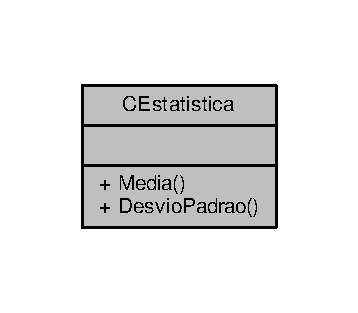
\includegraphics[width=172pt]{classCEstatistica__coll__graph}
\end{center}
\end{figure}
\subsection*{Public Member Functions}
\begin{DoxyCompactItemize}
\item 
\hypertarget{classCEstatistica_a9c0b46a34059ed41c94f1816808badd7}{double \hyperlink{classCEstatistica_a9c0b46a34059ed41c94f1816808badd7}{Media} (std\-::vector$<$ double $>$ v)}\label{classCEstatistica_a9c0b46a34059ed41c94f1816808badd7}

\begin{DoxyCompactList}\small\item\em retorna a media do vetor informado \end{DoxyCompactList}\item 
\hypertarget{classCEstatistica_ae7ad27a27293f6447160ca0f38c37559}{double \hyperlink{classCEstatistica_ae7ad27a27293f6447160ca0f38c37559}{Desvio\-Padrao} (std\-::vector$<$ double $>$ v)}\label{classCEstatistica_ae7ad27a27293f6447160ca0f38c37559}

\begin{DoxyCompactList}\small\item\em retorna o desvio padrao do vetor informado \end{DoxyCompactList}\end{DoxyCompactItemize}


\subsection{Detailed Description}
Classe que calcula estatisticas do vetor, como media e desvio padrao, util para regressao. 

The documentation for this class was generated from the following files\-:\begin{DoxyCompactItemize}
\item 
C\-Estatistica.\-h\item 
C\-Estatistica.\-cpp\end{DoxyCompactItemize}

\hypertarget{classCFluido}{\section{C\-Fluido Class Reference}
\label{classCFluido}\index{C\-Fluido@{C\-Fluido}}
}


Classe contendo as caracteristicas do fluido produzido.  




{\ttfamily \#include $<$C\-Fluido.\-h$>$}



Collaboration diagram for C\-Fluido\-:
\nopagebreak
\begin{figure}[H]
\begin{center}
\leavevmode
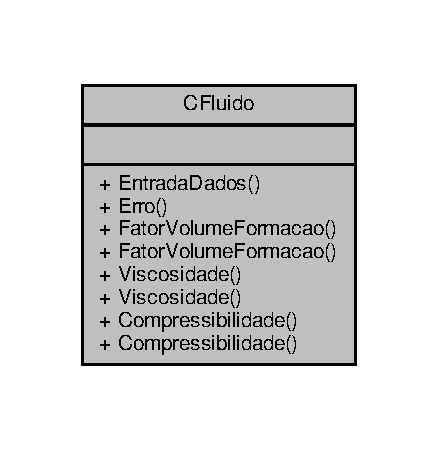
\includegraphics[width=210pt]{classCFluido__coll__graph}
\end{center}
\end{figure}
\subsection*{Public Member Functions}
\begin{DoxyCompactItemize}
\item 
void \hyperlink{classCFluido_a763eff2c0992744c8482beb56171981d}{Entrada\-Dados} ()
\item 
\hypertarget{classCFluido_a6262833c7f9a37dd886a1b8c5cf798d5}{void \hyperlink{classCFluido_a6262833c7f9a37dd886a1b8c5cf798d5}{Erro} ()}\label{classCFluido_a6262833c7f9a37dd886a1b8c5cf798d5}

\begin{DoxyCompactList}\small\item\em Funcao que verifica se houve erro na entrada de dados e pede nova entrada ate nao ocorrer erro. \end{DoxyCompactList}\item 
\hypertarget{classCFluido_ad8d3ec53a4cb37b3824ec3d64a49c2bc}{void \hyperlink{classCFluido_ad8d3ec53a4cb37b3824ec3d64a49c2bc}{Fator\-Volume\-Formacao} (double \-\_\-fator\-Volume\-Formacao)}\label{classCFluido_ad8d3ec53a4cb37b3824ec3d64a49c2bc}

\begin{DoxyCompactList}\small\item\em Funcao que seta o fatorvolumeformacao. \end{DoxyCompactList}\item 
\hypertarget{classCFluido_aac30ac0af8dfa17bfdaacff472351054}{double \hyperlink{classCFluido_aac30ac0af8dfa17bfdaacff472351054}{Fator\-Volume\-Formacao} () const }\label{classCFluido_aac30ac0af8dfa17bfdaacff472351054}

\begin{DoxyCompactList}\small\item\em Funcao get do fatorvolumeformacao. \end{DoxyCompactList}\item 
\hypertarget{classCFluido_a4523b55aae9b4721de73def751cdb078}{void \hyperlink{classCFluido_a4523b55aae9b4721de73def751cdb078}{Viscosidade} (double \-\_\-viscosidade)}\label{classCFluido_a4523b55aae9b4721de73def751cdb078}

\begin{DoxyCompactList}\small\item\em Funcao que seta a viscosidade. \end{DoxyCompactList}\item 
\hypertarget{classCFluido_ac134bfe73c9e96643cc5e3a59fd658a8}{double \hyperlink{classCFluido_ac134bfe73c9e96643cc5e3a59fd658a8}{Viscosidade} () const }\label{classCFluido_ac134bfe73c9e96643cc5e3a59fd658a8}

\begin{DoxyCompactList}\small\item\em Funcao get da viscosidade. \end{DoxyCompactList}\item 
\hypertarget{classCFluido_aca95a551083d35ff51792bb622517ce5}{void \hyperlink{classCFluido_aca95a551083d35ff51792bb622517ce5}{Compressibilidade} (double \-\_\-compressibilidade)}\label{classCFluido_aca95a551083d35ff51792bb622517ce5}

\begin{DoxyCompactList}\small\item\em Funcao que seta a compressibilidade. \end{DoxyCompactList}\item 
\hypertarget{classCFluido_a8ab2fc5851cc7e8ad6c55c3af7856f19}{double \hyperlink{classCFluido_a8ab2fc5851cc7e8ad6c55c3af7856f19}{Compressibilidade} () const }\label{classCFluido_a8ab2fc5851cc7e8ad6c55c3af7856f19}

\begin{DoxyCompactList}\small\item\em Funcao get da compressibilidade. \end{DoxyCompactList}\end{DoxyCompactItemize}


\subsection{Detailed Description}
Classe contendo as caracteristicas do fluido produzido. 

\subsection{Member Function Documentation}
\hypertarget{classCFluido_a763eff2c0992744c8482beb56171981d}{\index{C\-Fluido@{C\-Fluido}!Entrada\-Dados@{Entrada\-Dados}}
\index{Entrada\-Dados@{Entrada\-Dados}!CFluido@{C\-Fluido}}
\subsubsection[{Entrada\-Dados}]{\setlength{\rightskip}{0pt plus 5cm}void C\-Fluido\-::\-Entrada\-Dados (
\begin{DoxyParamCaption}
{}
\end{DoxyParamCaption}
)}}\label{classCFluido_a763eff2c0992744c8482beb56171981d}
Funcao que recebe dados do usuario, preenchendo atributos fatorvolumeformacao, viscosidade, compressibilidade 

The documentation for this class was generated from the following files\-:\begin{DoxyCompactItemize}
\item 
C\-Fluido.\-h\item 
C\-Fluido.\-cpp\end{DoxyCompactItemize}

\hypertarget{classCPoco}{\section{C\-Poco Class Reference}
\label{classCPoco}\index{C\-Poco@{C\-Poco}}
}


Classe contendo as caracteristicas do poco.  




{\ttfamily \#include $<$C\-Poco.\-h$>$}



Collaboration diagram for C\-Poco\-:
\nopagebreak
\begin{figure}[H]
\begin{center}
\leavevmode
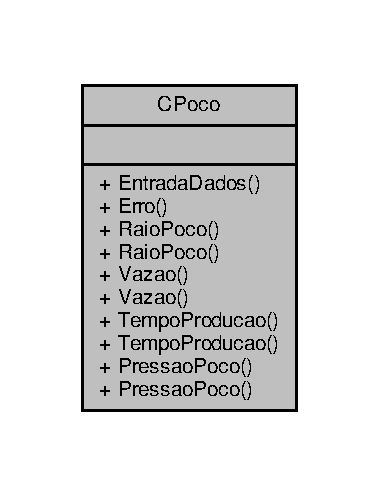
\includegraphics[width=182pt]{classCPoco__coll__graph}
\end{center}
\end{figure}
\subsection*{Public Member Functions}
\begin{DoxyCompactItemize}
\item 
\hypertarget{classCPoco_aa1e23aefdb4a4efbc4cef7a5d5306f2c}{void \hyperlink{classCPoco_aa1e23aefdb4a4efbc4cef7a5d5306f2c}{Entrada\-Dados} ()}\label{classCPoco_aa1e23aefdb4a4efbc4cef7a5d5306f2c}

\begin{DoxyCompactList}\small\item\em Funcao que recebe dados do usuario, preenchendo atributos raiopoco, vazao, tempoproducao, pressaopoco. \end{DoxyCompactList}\item 
\hypertarget{classCPoco_a5de538de21fc145866380e35bd9f484a}{void \hyperlink{classCPoco_a5de538de21fc145866380e35bd9f484a}{Erro} ()}\label{classCPoco_a5de538de21fc145866380e35bd9f484a}

\begin{DoxyCompactList}\small\item\em Funcao que verifica se houve erro na entrada de dados e pede nova entrada ate nao ocorrer erro. \end{DoxyCompactList}\item 
\hypertarget{classCPoco_a19879337015fdec5dcfc5aec710244e1}{void \hyperlink{classCPoco_a19879337015fdec5dcfc5aec710244e1}{Raio\-Poco} (double \-\_\-raio\-Poco)}\label{classCPoco_a19879337015fdec5dcfc5aec710244e1}

\begin{DoxyCompactList}\small\item\em Funcao que seta o raiopoco. \end{DoxyCompactList}\item 
\hypertarget{classCPoco_ad773ade15b096fde9b369f2199acfca1}{double \hyperlink{classCPoco_ad773ade15b096fde9b369f2199acfca1}{Raio\-Poco} () const }\label{classCPoco_ad773ade15b096fde9b369f2199acfca1}

\begin{DoxyCompactList}\small\item\em Funcao get do raiopoco. \end{DoxyCompactList}\item 
\hypertarget{classCPoco_a5d957a20d22b97515c726862a2b5e870}{void \hyperlink{classCPoco_a5d957a20d22b97515c726862a2b5e870}{Vazao} (double \-\_\-vazao)}\label{classCPoco_a5d957a20d22b97515c726862a2b5e870}

\begin{DoxyCompactList}\small\item\em Funcao que seta a vazao. \end{DoxyCompactList}\item 
\hypertarget{classCPoco_a2988747a01ebf170e1ca56d407e2c5c6}{double \hyperlink{classCPoco_a2988747a01ebf170e1ca56d407e2c5c6}{Vazao} () const }\label{classCPoco_a2988747a01ebf170e1ca56d407e2c5c6}

\begin{DoxyCompactList}\small\item\em Funcao get da vazao. \end{DoxyCompactList}\item 
\hypertarget{classCPoco_a0458cc7f91feb48f0d925f3075eaad5f}{void \hyperlink{classCPoco_a0458cc7f91feb48f0d925f3075eaad5f}{Tempo\-Producao} (double \-\_\-tempo\-Producao)}\label{classCPoco_a0458cc7f91feb48f0d925f3075eaad5f}

\begin{DoxyCompactList}\small\item\em Funcao que seta o tempoproducao. \end{DoxyCompactList}\item 
\hypertarget{classCPoco_aa416c03fa3d259322d5a015dff4b1d98}{double \hyperlink{classCPoco_aa416c03fa3d259322d5a015dff4b1d98}{Tempo\-Producao} () const }\label{classCPoco_aa416c03fa3d259322d5a015dff4b1d98}

\begin{DoxyCompactList}\small\item\em Funcao get do tempoproducao. \end{DoxyCompactList}\item 
\hypertarget{classCPoco_a5c0737c83668c9d6e0e40685bed11472}{void \hyperlink{classCPoco_a5c0737c83668c9d6e0e40685bed11472}{Pressao\-Poco} (double \-\_\-pressao\-Poco)}\label{classCPoco_a5c0737c83668c9d6e0e40685bed11472}

\begin{DoxyCompactList}\small\item\em Funcao que seta a pressaopoco. \end{DoxyCompactList}\item 
\hypertarget{classCPoco_a570c72af4e2f331bfb3236dcc09161bf}{double \hyperlink{classCPoco_a570c72af4e2f331bfb3236dcc09161bf}{Pressao\-Poco} () const }\label{classCPoco_a570c72af4e2f331bfb3236dcc09161bf}

\begin{DoxyCompactList}\small\item\em Funcao get da pressaopoco. \end{DoxyCompactList}\end{DoxyCompactItemize}


\subsection{Detailed Description}
Classe contendo as caracteristicas do poco. 

The documentation for this class was generated from the following files\-:\begin{DoxyCompactItemize}
\item 
C\-Poco.\-h\item 
C\-Poco.\-cpp\end{DoxyCompactItemize}

\hypertarget{classCReservatorio}{\section{C\-Reservatorio Class Reference}
\label{classCReservatorio}\index{C\-Reservatorio@{C\-Reservatorio}}
}


Classe contendo as caracteristicas do reservatorio.  




{\ttfamily \#include $<$C\-Reservatorio.\-h$>$}



Collaboration diagram for C\-Reservatorio\-:
\nopagebreak
\begin{figure}[H]
\begin{center}
\leavevmode
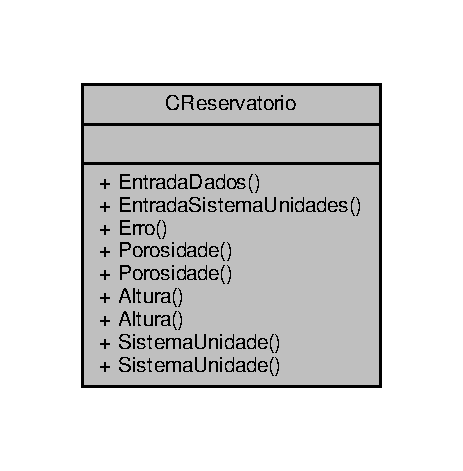
\includegraphics[width=222pt]{classCReservatorio__coll__graph}
\end{center}
\end{figure}
\subsection*{Public Member Functions}
\begin{DoxyCompactItemize}
\item 
\hypertarget{classCReservatorio_af97e48ff5b4409f8e3f85751731373cd}{void \hyperlink{classCReservatorio_af97e48ff5b4409f8e3f85751731373cd}{Entrada\-Dados} ()}\label{classCReservatorio_af97e48ff5b4409f8e3f85751731373cd}

\begin{DoxyCompactList}\small\item\em Funcao que recebe dados do usuario, preenchendo atributos porosidade e altura. \end{DoxyCompactList}\item 
\hypertarget{classCReservatorio_aade83e0ca5f8a58bc20912377dc4b9ee}{void \hyperlink{classCReservatorio_aade83e0ca5f8a58bc20912377dc4b9ee}{Entrada\-Sistema\-Unidades} ()}\label{classCReservatorio_aade83e0ca5f8a58bc20912377dc4b9ee}

\begin{DoxyCompactList}\small\item\em Funcao que exibe um menu e recebe dado do usuario, esse dado preenche o atributo sistemaunidade. \end{DoxyCompactList}\item 
\hypertarget{classCReservatorio_a988c1fec6af707261b008e2f1ec74bea}{void \hyperlink{classCReservatorio_a988c1fec6af707261b008e2f1ec74bea}{Erro} ()}\label{classCReservatorio_a988c1fec6af707261b008e2f1ec74bea}

\begin{DoxyCompactList}\small\item\em Funcao que verifica se houve erro na entrada de dados e pede nova entrada ate nao ocorrer erro. \end{DoxyCompactList}\item 
\hypertarget{classCReservatorio_af50a6fd17a916fcb4835b263bb46d344}{void \hyperlink{classCReservatorio_af50a6fd17a916fcb4835b263bb46d344}{Porosidade} (double \-\_\-porosidade)}\label{classCReservatorio_af50a6fd17a916fcb4835b263bb46d344}

\begin{DoxyCompactList}\small\item\em Funcao que seta a porosidade. \end{DoxyCompactList}\item 
\hypertarget{classCReservatorio_a1f0524cd7b9439e2c13908658fcb5317}{double \hyperlink{classCReservatorio_a1f0524cd7b9439e2c13908658fcb5317}{Porosidade} () const }\label{classCReservatorio_a1f0524cd7b9439e2c13908658fcb5317}

\begin{DoxyCompactList}\small\item\em Funcao get da porosidade. \end{DoxyCompactList}\item 
\hypertarget{classCReservatorio_a446c0a9088655695a7180f0a6444d5a7}{void \hyperlink{classCReservatorio_a446c0a9088655695a7180f0a6444d5a7}{Altura} (double \-\_\-altura)}\label{classCReservatorio_a446c0a9088655695a7180f0a6444d5a7}

\begin{DoxyCompactList}\small\item\em Funcao que seta a altura. \end{DoxyCompactList}\item 
\hypertarget{classCReservatorio_a99c3dba3632785a5f392776c4f5a35cb}{double \hyperlink{classCReservatorio_a99c3dba3632785a5f392776c4f5a35cb}{Altura} () const }\label{classCReservatorio_a99c3dba3632785a5f392776c4f5a35cb}

\begin{DoxyCompactList}\small\item\em Funcao get da porosidade. \end{DoxyCompactList}\item 
\hypertarget{classCReservatorio_a2444dd4eccc764e132d2451651f7a658}{void \hyperlink{classCReservatorio_a2444dd4eccc764e132d2451651f7a658}{Sistema\-Unidade} (double \-\_\-sistema\-Unidade)}\label{classCReservatorio_a2444dd4eccc764e132d2451651f7a658}

\begin{DoxyCompactList}\small\item\em Funcao que seta o sistemaunidade. \end{DoxyCompactList}\item 
\hypertarget{classCReservatorio_a9d45fb13dd53281fc2de9ea5b4a3f44b}{double \hyperlink{classCReservatorio_a9d45fb13dd53281fc2de9ea5b4a3f44b}{Sistema\-Unidade} () const }\label{classCReservatorio_a9d45fb13dd53281fc2de9ea5b4a3f44b}

\begin{DoxyCompactList}\small\item\em Funcao get do sistemaunidade. \end{DoxyCompactList}\end{DoxyCompactItemize}


\subsection{Detailed Description}
Classe contendo as caracteristicas do reservatorio. 

The documentation for this class was generated from the following files\-:\begin{DoxyCompactItemize}
\item 
C\-Reservatorio.\-h\item 
C\-Reservatorio.\-cpp\end{DoxyCompactItemize}

\hypertarget{classCSimuladorAnaliseTestePressao}{\section{C\-Simulador\-Analise\-Teste\-Pressao Class Reference}
\label{classCSimuladorAnaliseTestePressao}\index{C\-Simulador\-Analise\-Teste\-Pressao@{C\-Simulador\-Analise\-Teste\-Pressao}}
}


Classe que faz a analise do teste de pressao realizado no campo e infere as propriedades do reservatorio.  




{\ttfamily \#include $<$C\-Simulador\-Analise\-Teste\-Pressao.\-h$>$}



Collaboration diagram for C\-Simulador\-Analise\-Teste\-Pressao\-:
\nopagebreak
\begin{figure}[H]
\begin{center}
\leavevmode
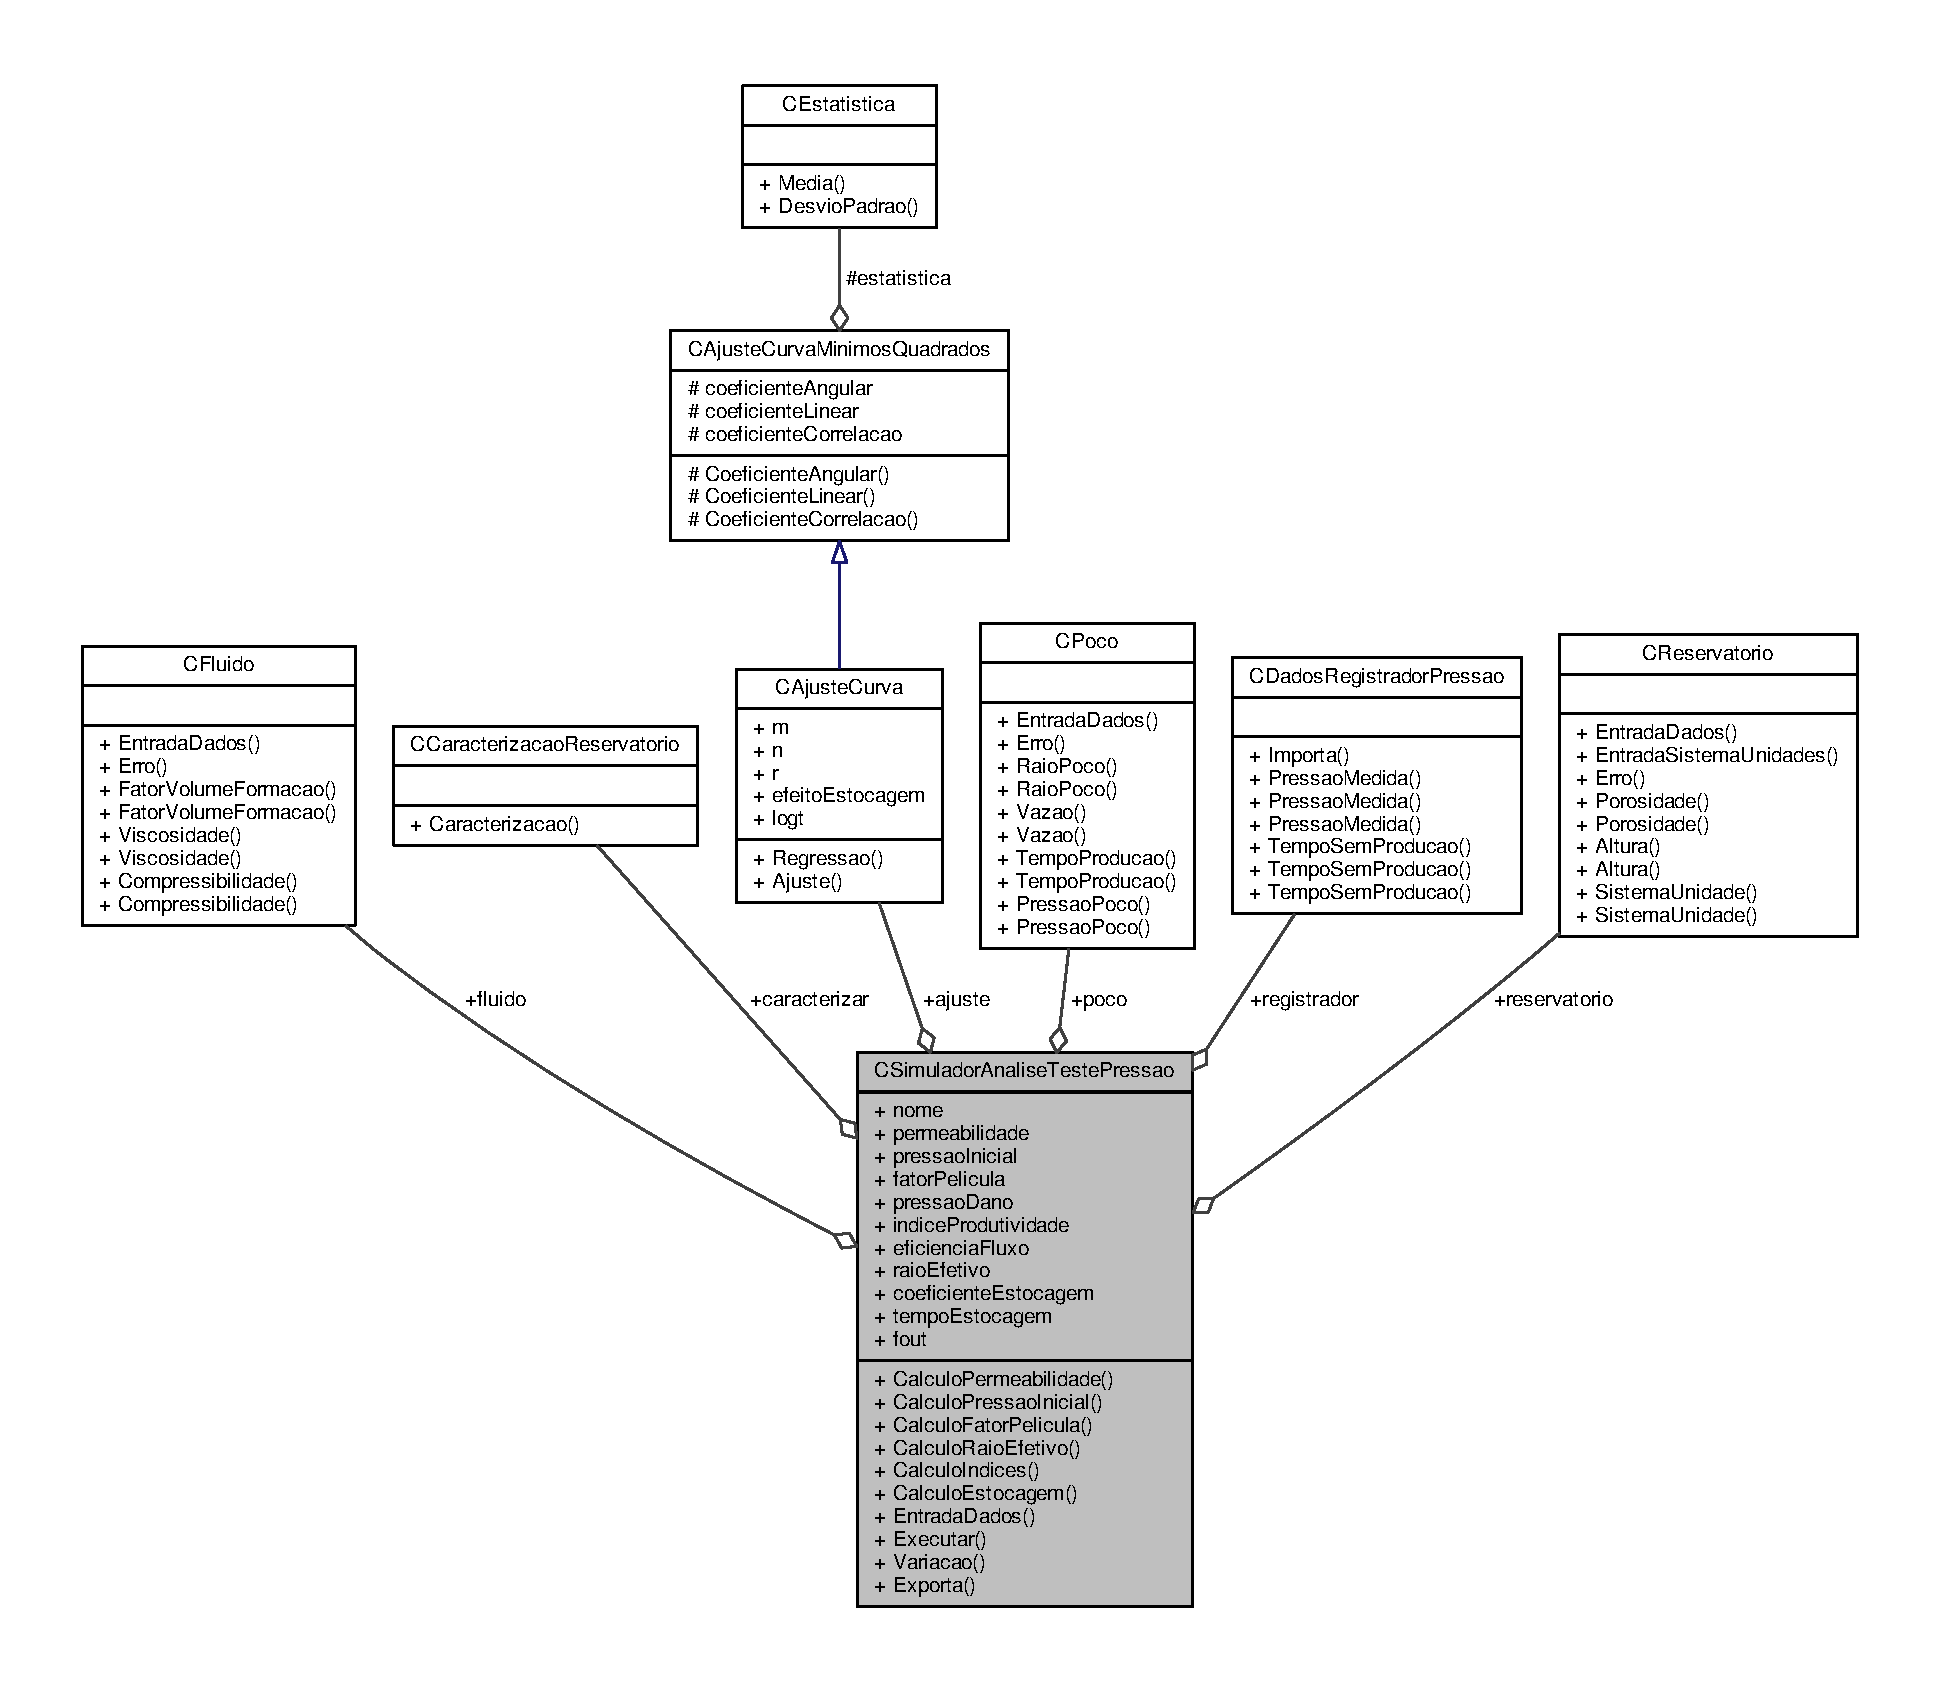
\includegraphics[width=350pt]{classCSimuladorAnaliseTestePressao__coll__graph}
\end{center}
\end{figure}
\subsection*{Public Member Functions}
\begin{DoxyCompactItemize}
\item 
void \hyperlink{classCSimuladorAnaliseTestePressao_aefe1ad8908c9f3b7e48d9549675d8e14}{Calculo\-Permeabilidade} ()
\begin{DoxyCompactList}\small\item\em criacao do objeto plot da classe C\-Gnuplot \end{DoxyCompactList}\item 
\hypertarget{classCSimuladorAnaliseTestePressao_a2e8d3841dd1f0215ad21787138c7eb78}{void \hyperlink{classCSimuladorAnaliseTestePressao_a2e8d3841dd1f0215ad21787138c7eb78}{Calculo\-Pressao\-Inicial} ()}\label{classCSimuladorAnaliseTestePressao_a2e8d3841dd1f0215ad21787138c7eb78}

\begin{DoxyCompactList}\small\item\em Funcao que calcula e preenche o atributo pressaoinicial. \end{DoxyCompactList}\item 
\hypertarget{classCSimuladorAnaliseTestePressao_a61dc2ce4a3106aac530b64f5ab5cf30d}{void \hyperlink{classCSimuladorAnaliseTestePressao_a61dc2ce4a3106aac530b64f5ab5cf30d}{Calculo\-Fator\-Pelicula} ()}\label{classCSimuladorAnaliseTestePressao_a61dc2ce4a3106aac530b64f5ab5cf30d}

\begin{DoxyCompactList}\small\item\em Funcao que calcula e preenche o atributo fatorpelicula. \end{DoxyCompactList}\item 
\hypertarget{classCSimuladorAnaliseTestePressao_aa2f3fa25f3db3ca4c65d8b854e004781}{void \hyperlink{classCSimuladorAnaliseTestePressao_aa2f3fa25f3db3ca4c65d8b854e004781}{Calculo\-Raio\-Efetivo} ()}\label{classCSimuladorAnaliseTestePressao_aa2f3fa25f3db3ca4c65d8b854e004781}

\begin{DoxyCompactList}\small\item\em Funcao que calcula e preenche o atributo raioefetivo. \end{DoxyCompactList}\item 
\hypertarget{classCSimuladorAnaliseTestePressao_a5683325b63f4f55886a39a1495539219}{void \hyperlink{classCSimuladorAnaliseTestePressao_a5683325b63f4f55886a39a1495539219}{Calculo\-Indices} ()}\label{classCSimuladorAnaliseTestePressao_a5683325b63f4f55886a39a1495539219}

\begin{DoxyCompactList}\small\item\em Funcao que calcula e preenche os atributos indiceprodutividade, eficienciafluxo, pressaodano. \end{DoxyCompactList}\item 
\hypertarget{classCSimuladorAnaliseTestePressao_a89bd4fd7284643a2b36b219ba250b8da}{void \hyperlink{classCSimuladorAnaliseTestePressao_a89bd4fd7284643a2b36b219ba250b8da}{Calculo\-Estocagem} ()}\label{classCSimuladorAnaliseTestePressao_a89bd4fd7284643a2b36b219ba250b8da}

\begin{DoxyCompactList}\small\item\em Funcao que calcula e preenche os atributos coeficienteestocagem e tempoestocagem. \end{DoxyCompactList}\item 
\hypertarget{classCSimuladorAnaliseTestePressao_ac8a12e3680c2d53c47083d27940ecf4c}{void \hyperlink{classCSimuladorAnaliseTestePressao_ac8a12e3680c2d53c47083d27940ecf4c}{Entrada\-Dados} ()}\label{classCSimuladorAnaliseTestePressao_ac8a12e3680c2d53c47083d27940ecf4c}

\begin{DoxyCompactList}\small\item\em Funcao que chama as entradas de dados necessarias. \end{DoxyCompactList}\item 
\hypertarget{classCSimuladorAnaliseTestePressao_a1a3fc00da83a0a1e05b1f7d94dd600ba}{void \hyperlink{classCSimuladorAnaliseTestePressao_a1a3fc00da83a0a1e05b1f7d94dd600ba}{Executar} ()}\label{classCSimuladorAnaliseTestePressao_a1a3fc00da83a0a1e05b1f7d94dd600ba}

\begin{DoxyCompactList}\small\item\em Funcao principal que executa a simulacao do teste. \end{DoxyCompactList}\item 
void \hyperlink{classCSimuladorAnaliseTestePressao_a2069ce0bab92d9b21413a713da2a090f}{Variacao} ()
\begin{DoxyCompactList}\small\item\em Varia parametros de reservatorio. \end{DoxyCompactList}\item 
void \hyperlink{classCSimuladorAnaliseTestePressao_aa88d01ae70a4dcd4280e78101da4f3c4}{Exporta} ()
\begin{DoxyCompactList}\small\item\em Funcao que exporta os dados para um arquivo.\-dat. \end{DoxyCompactList}\end{DoxyCompactItemize}
\subsection*{Public Attributes}
\begin{DoxyCompactItemize}
\item 
\hypertarget{classCSimuladorAnaliseTestePressao_a840551f5e6d796b18f3036ba721563ee}{std\-::string \hyperlink{classCSimuladorAnaliseTestePressao_a840551f5e6d796b18f3036ba721563ee}{nome}}\label{classCSimuladorAnaliseTestePressao_a840551f5e6d796b18f3036ba721563ee}

\begin{DoxyCompactList}\small\item\em Nome do Arquivo exportado. \end{DoxyCompactList}\item 
\hypertarget{classCSimuladorAnaliseTestePressao_a19204e4ede4f658c53349e794382e542}{double \hyperlink{classCSimuladorAnaliseTestePressao_a19204e4ede4f658c53349e794382e542}{permeabilidade}}\label{classCSimuladorAnaliseTestePressao_a19204e4ede4f658c53349e794382e542}

\begin{DoxyCompactList}\small\item\em permeabilidade do reservatorio \end{DoxyCompactList}\item 
\hypertarget{classCSimuladorAnaliseTestePressao_a695f33f39e0bb2757c4cae1bfc1b3bd1}{double \hyperlink{classCSimuladorAnaliseTestePressao_a695f33f39e0bb2757c4cae1bfc1b3bd1}{pressao\-Inicial}}\label{classCSimuladorAnaliseTestePressao_a695f33f39e0bb2757c4cae1bfc1b3bd1}

\begin{DoxyCompactList}\small\item\em pressao inicial que se encontrava o reservatorio \end{DoxyCompactList}\item 
\hypertarget{classCSimuladorAnaliseTestePressao_ab528258b33e70123fa4767af665dba63}{double \hyperlink{classCSimuladorAnaliseTestePressao_ab528258b33e70123fa4767af665dba63}{fator\-Pelicula}}\label{classCSimuladorAnaliseTestePressao_ab528258b33e70123fa4767af665dba63}

\begin{DoxyCompactList}\small\item\em skin factor do poco \end{DoxyCompactList}\item 
\hypertarget{classCSimuladorAnaliseTestePressao_af666fb2636ecca426b94f600d627fa7e}{double \hyperlink{classCSimuladorAnaliseTestePressao_af666fb2636ecca426b94f600d627fa7e}{pressao\-Dano}}\label{classCSimuladorAnaliseTestePressao_af666fb2636ecca426b94f600d627fa7e}

\begin{DoxyCompactList}\small\item\em queda de pressao referente ao fator de pelicula \end{DoxyCompactList}\item 
\hypertarget{classCSimuladorAnaliseTestePressao_af06a4adbc5b0a5b24108d270104415e8}{double \hyperlink{classCSimuladorAnaliseTestePressao_af06a4adbc5b0a5b24108d270104415e8}{indice\-Produtividade}}\label{classCSimuladorAnaliseTestePressao_af06a4adbc5b0a5b24108d270104415e8}

\begin{DoxyCompactList}\small\item\em indice de produtividade do reservatorio \end{DoxyCompactList}\item 
\hypertarget{classCSimuladorAnaliseTestePressao_a773c3fd731511ff73f403c0fabef8d40}{double \hyperlink{classCSimuladorAnaliseTestePressao_a773c3fd731511ff73f403c0fabef8d40}{eficiencia\-Fluxo}}\label{classCSimuladorAnaliseTestePressao_a773c3fd731511ff73f403c0fabef8d40}

\begin{DoxyCompactList}\small\item\em eficiencia de fluxo do reservatorio \end{DoxyCompactList}\item 
\hypertarget{classCSimuladorAnaliseTestePressao_afeaf2313fbcb992542ad5f71588ff990}{double \hyperlink{classCSimuladorAnaliseTestePressao_afeaf2313fbcb992542ad5f71588ff990}{raio\-Efetivo}}\label{classCSimuladorAnaliseTestePressao_afeaf2313fbcb992542ad5f71588ff990}

\begin{DoxyCompactList}\small\item\em raio efetivo do poco \end{DoxyCompactList}\item 
\hypertarget{classCSimuladorAnaliseTestePressao_ae6e622fa4af0eeda667c626cd8ddf5a8}{double \hyperlink{classCSimuladorAnaliseTestePressao_ae6e622fa4af0eeda667c626cd8ddf5a8}{coeficiente\-Estocagem}}\label{classCSimuladorAnaliseTestePressao_ae6e622fa4af0eeda667c626cd8ddf5a8}

\begin{DoxyCompactList}\small\item\em coeficiente de estocagem do poco \end{DoxyCompactList}\item 
\hypertarget{classCSimuladorAnaliseTestePressao_a4d9eeeca9c091b858ccd8a709f4a02d0}{double \hyperlink{classCSimuladorAnaliseTestePressao_a4d9eeeca9c091b858ccd8a709f4a02d0}{tempo\-Estocagem}}\label{classCSimuladorAnaliseTestePressao_a4d9eeeca9c091b858ccd8a709f4a02d0}

\begin{DoxyCompactList}\small\item\em tempo de duracao do efeito de estocagem \end{DoxyCompactList}\item 
\hypertarget{classCSimuladorAnaliseTestePressao_aa143509a0af5103d4be29863e71c33c6}{std\-::ofstream \hyperlink{classCSimuladorAnaliseTestePressao_aa143509a0af5103d4be29863e71c33c6}{fout}}\label{classCSimuladorAnaliseTestePressao_aa143509a0af5103d4be29863e71c33c6}

\begin{DoxyCompactList}\small\item\em cria objeto de armazenamento de dados \end{DoxyCompactList}\item 
\hypertarget{classCSimuladorAnaliseTestePressao_acd63655a60e5822852b0f94b44a85169}{\hyperlink{classCPoco}{C\-Poco} \hyperlink{classCSimuladorAnaliseTestePressao_acd63655a60e5822852b0f94b44a85169}{poco}}\label{classCSimuladorAnaliseTestePressao_acd63655a60e5822852b0f94b44a85169}

\begin{DoxyCompactList}\small\item\em criacao do objeto poco da classe \hyperlink{classCPoco}{C\-Poco} \end{DoxyCompactList}\item 
\hypertarget{classCSimuladorAnaliseTestePressao_a94e2a61bbe5f76dca90a44e477635af8}{\hyperlink{classCFluido}{C\-Fluido} \hyperlink{classCSimuladorAnaliseTestePressao_a94e2a61bbe5f76dca90a44e477635af8}{fluido}}\label{classCSimuladorAnaliseTestePressao_a94e2a61bbe5f76dca90a44e477635af8}

\begin{DoxyCompactList}\small\item\em criacao do objeto fluido da classe \hyperlink{classCFluido}{C\-Fluido} \end{DoxyCompactList}\item 
\hypertarget{classCSimuladorAnaliseTestePressao_a4d52ce30c56b27d961fd4b4e93c86ebb}{\hyperlink{classCReservatorio}{C\-Reservatorio} \hyperlink{classCSimuladorAnaliseTestePressao_a4d52ce30c56b27d961fd4b4e93c86ebb}{reservatorio}}\label{classCSimuladorAnaliseTestePressao_a4d52ce30c56b27d961fd4b4e93c86ebb}

\begin{DoxyCompactList}\small\item\em criacao do objeto reservatorio da classe \hyperlink{classCReservatorio}{C\-Reservatorio} \end{DoxyCompactList}\item 
\hypertarget{classCSimuladorAnaliseTestePressao_aa7bbb2d46909207f38fb3b1b4ce9730a}{\hyperlink{classCDadosRegistradorPressao}{C\-Dados\-Registrador\-Pressao} \hyperlink{classCSimuladorAnaliseTestePressao_aa7bbb2d46909207f38fb3b1b4ce9730a}{registrador}}\label{classCSimuladorAnaliseTestePressao_aa7bbb2d46909207f38fb3b1b4ce9730a}

\begin{DoxyCompactList}\small\item\em criacao do objeto registrador da classe C\-Registrador \end{DoxyCompactList}\item 
\hypertarget{classCSimuladorAnaliseTestePressao_a4b2ab614049cad5c31ca00cdcd8c2bce}{\hyperlink{classCAjusteCurva}{C\-Ajuste\-Curva} \hyperlink{classCSimuladorAnaliseTestePressao_a4b2ab614049cad5c31ca00cdcd8c2bce}{ajuste}}\label{classCSimuladorAnaliseTestePressao_a4b2ab614049cad5c31ca00cdcd8c2bce}

\begin{DoxyCompactList}\small\item\em criacao do objeto ajuste da classe C\-Ajuste \end{DoxyCompactList}\item 
\hypertarget{classCSimuladorAnaliseTestePressao_af53097309b69539f55478b35d8aa9c0e}{\hyperlink{classCCaracterizacaoReservatorio}{C\-Caracterizacao\-Reservatorio} \hyperlink{classCSimuladorAnaliseTestePressao_af53097309b69539f55478b35d8aa9c0e}{caracterizar}}\label{classCSimuladorAnaliseTestePressao_af53097309b69539f55478b35d8aa9c0e}

\begin{DoxyCompactList}\small\item\em criacao do objeto caracterizar da classe C\-Caracterizacao \end{DoxyCompactList}\end{DoxyCompactItemize}


\subsection{Detailed Description}
Classe que faz a analise do teste de pressao realizado no campo e infere as propriedades do reservatorio. 

\subsection{Member Function Documentation}
\hypertarget{classCSimuladorAnaliseTestePressao_aefe1ad8908c9f3b7e48d9549675d8e14}{\index{C\-Simulador\-Analise\-Teste\-Pressao@{C\-Simulador\-Analise\-Teste\-Pressao}!Calculo\-Permeabilidade@{Calculo\-Permeabilidade}}
\index{Calculo\-Permeabilidade@{Calculo\-Permeabilidade}!CSimuladorAnaliseTestePressao@{C\-Simulador\-Analise\-Teste\-Pressao}}
\subsubsection[{Calculo\-Permeabilidade}]{\setlength{\rightskip}{0pt plus 5cm}void C\-Simulador\-Analise\-Teste\-Pressao\-::\-Calculo\-Permeabilidade (
\begin{DoxyParamCaption}
{}
\end{DoxyParamCaption}
)}}\label{classCSimuladorAnaliseTestePressao_aefe1ad8908c9f3b7e48d9549675d8e14}


criacao do objeto plot da classe C\-Gnuplot 

Funcao que calcula e preenche o atributo permeabilidade criacao do objeto armazena da classe \hyperlink{classCSimuladorAnaliseTestePressao}{C\-Simulador\-Analise\-Teste\-Pressao} \hypertarget{classCSimuladorAnaliseTestePressao_aa88d01ae70a4dcd4280e78101da4f3c4}{\index{C\-Simulador\-Analise\-Teste\-Pressao@{C\-Simulador\-Analise\-Teste\-Pressao}!Exporta@{Exporta}}
\index{Exporta@{Exporta}!CSimuladorAnaliseTestePressao@{C\-Simulador\-Analise\-Teste\-Pressao}}
\subsubsection[{Exporta}]{\setlength{\rightskip}{0pt plus 5cm}void C\-Simulador\-Analise\-Teste\-Pressao\-::\-Exporta (
\begin{DoxyParamCaption}
{}
\end{DoxyParamCaption}
)}}\label{classCSimuladorAnaliseTestePressao_aa88d01ae70a4dcd4280e78101da4f3c4}


Funcao que exporta os dados para um arquivo.\-dat. 

abre aquivo

criacao do objeto armazena da classe \hyperlink{classCSimuladorAnaliseTestePressao}{C\-Simulador\-Analise\-Teste\-Pressao} \hypertarget{classCSimuladorAnaliseTestePressao_a2069ce0bab92d9b21413a713da2a090f}{\index{C\-Simulador\-Analise\-Teste\-Pressao@{C\-Simulador\-Analise\-Teste\-Pressao}!Variacao@{Variacao}}
\index{Variacao@{Variacao}!CSimuladorAnaliseTestePressao@{C\-Simulador\-Analise\-Teste\-Pressao}}
\subsubsection[{Variacao}]{\setlength{\rightskip}{0pt plus 5cm}void C\-Simulador\-Analise\-Teste\-Pressao\-::\-Variacao (
\begin{DoxyParamCaption}
{}
\end{DoxyParamCaption}
)}}\label{classCSimuladorAnaliseTestePressao_a2069ce0bab92d9b21413a713da2a090f}


Varia parametros de reservatorio. 

abre aquivo

criacao do objeto armazena da classe \hyperlink{classCSimuladorAnaliseTestePressao}{C\-Simulador\-Analise\-Teste\-Pressao}

abre aquivo

criacao do objeto armazena da classe \hyperlink{classCSimuladorAnaliseTestePressao}{C\-Simulador\-Analise\-Teste\-Pressao}

abre aquivo

criacao do objeto armazena da classe \hyperlink{classCSimuladorAnaliseTestePressao}{C\-Simulador\-Analise\-Teste\-Pressao}

abre aquivo

criacao do objeto armazena da classe \hyperlink{classCSimuladorAnaliseTestePressao}{C\-Simulador\-Analise\-Teste\-Pressao} 

The documentation for this class was generated from the following files\-:\begin{DoxyCompactItemize}
\item 
C\-Simulador\-Analise\-Teste\-Pressao.\-h\item 
C\-Simulador\-Analise\-Teste\-Pressao.\-cpp\end{DoxyCompactItemize}

\hypertarget{classGnuplot}{\section{Gnuplot Class Reference}
\label{classGnuplot}\index{Gnuplot@{Gnuplot}}
}


Classe de interface para acesso ao programa gnuplot.  




{\ttfamily \#include $<$cgnuplot.\-h$>$}



Collaboration diagram for Gnuplot\-:
\nopagebreak
\begin{figure}[H]
\begin{center}
\leavevmode
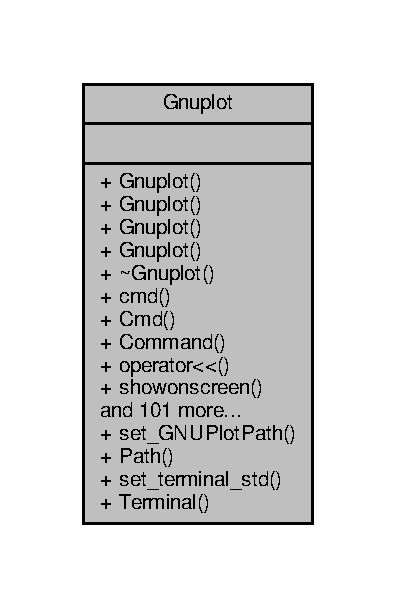
\includegraphics[width=190pt]{classGnuplot__coll__graph}
\end{center}
\end{figure}
\subsection*{Public Member Functions}
\begin{DoxyCompactItemize}
\item 
\hypertarget{classGnuplot_a187eb517b362cf379492fe7f1621ee50}{\hyperlink{classGnuplot_a187eb517b362cf379492fe7f1621ee50}{Gnuplot} (const std\-::string \&style=\char`\"{}points\char`\"{})}\label{classGnuplot_a187eb517b362cf379492fe7f1621ee50}

\begin{DoxyCompactList}\small\item\em Construtor, seta o estilo do grafico na construcao. \end{DoxyCompactList}\item 
\hypertarget{classGnuplot_a8ceac5808e42665c1dee305ae7ea9070}{\hyperlink{classGnuplot_a8ceac5808e42665c1dee305ae7ea9070}{Gnuplot} (const std\-::vector$<$ double $>$ \&x, const std\-::string \&title=\char`\"{}\char`\"{}, const std\-::string \&style=\char`\"{}points\char`\"{}, const std\-::string \&labelx=\char`\"{}x\char`\"{}, const std\-::string \&labely=\char`\"{}y\char`\"{})}\label{classGnuplot_a8ceac5808e42665c1dee305ae7ea9070}

\begin{DoxyCompactList}\small\item\em Construtor, plota um grafico a partir dde um vector, diretamente na construcao. \end{DoxyCompactList}\item 
\hypertarget{classGnuplot_a24327b6116c71acdc195eadf665c67cb}{\hyperlink{classGnuplot_a24327b6116c71acdc195eadf665c67cb}{Gnuplot} (const std\-::vector$<$ double $>$ \&x, const std\-::vector$<$ double $>$ \&y, const std\-::string \&title=\char`\"{}\char`\"{}, const std\-::string \&style=\char`\"{}points\char`\"{}, const std\-::string \&labelx=\char`\"{}x\char`\"{}, const std\-::string \&labely=\char`\"{}y\char`\"{})}\label{classGnuplot_a24327b6116c71acdc195eadf665c67cb}

\begin{DoxyCompactList}\small\item\em Construtor, plota um grafico do tipo x\-\_\-y a partir de vetores, diretamente na construcao. \end{DoxyCompactList}\item 
\hypertarget{classGnuplot_a14191e89154f2716608f6907975cc012}{\hyperlink{classGnuplot_a14191e89154f2716608f6907975cc012}{Gnuplot} (const std\-::vector$<$ double $>$ \&x, const std\-::vector$<$ double $>$ \&y, const std\-::vector$<$ double $>$ \&z, const std\-::string \&title=\char`\"{}\char`\"{}, const std\-::string \&style=\char`\"{}points\char`\"{}, const std\-::string \&labelx=\char`\"{}x\char`\"{}, const std\-::string \&labely=\char`\"{}y\char`\"{}, const std\-::string \&labelz=\char`\"{}z\char`\"{})}\label{classGnuplot_a14191e89154f2716608f6907975cc012}

\begin{DoxyCompactList}\small\item\em Construtor, plota um grafico de x\-\_\-y\-\_\-z a partir de vetores, diretamente na construcao. \end{DoxyCompactList}\item 
\hypertarget{classGnuplot_a78a68f621caa87d1f34324fcd093c7bd}{\hyperlink{classGnuplot_a78a68f621caa87d1f34324fcd093c7bd}{$\sim$\-Gnuplot} ()}\label{classGnuplot_a78a68f621caa87d1f34324fcd093c7bd}

\begin{DoxyCompactList}\small\item\em Destrutor, necessario para deletar arquivos temporarios. \end{DoxyCompactList}\item 
\hypertarget{classGnuplot_a07607803ede8dd5416906df0a1924fc5}{\hyperlink{classGnuplot}{Gnuplot} \& \hyperlink{classGnuplot_a07607803ede8dd5416906df0a1924fc5}{cmd} (const std\-::string \&cmdstr)}\label{classGnuplot_a07607803ede8dd5416906df0a1924fc5}

\begin{DoxyCompactList}\small\item\em Envia comando para o gnuplot. \end{DoxyCompactList}\item 
\hypertarget{classGnuplot_af9ffb5b4c18cdf7c56e5c446f72e515d}{\hyperlink{classGnuplot}{Gnuplot} \& \hyperlink{classGnuplot_af9ffb5b4c18cdf7c56e5c446f72e515d}{Cmd} (const std\-::string \&cmdstr)}\label{classGnuplot_af9ffb5b4c18cdf7c56e5c446f72e515d}

\begin{DoxyCompactList}\small\item\em Envia comando para o gnuplot. \end{DoxyCompactList}\item 
\hypertarget{classGnuplot_a0d6db1521e789d7b73415ce85b723046}{\hyperlink{classGnuplot}{Gnuplot} \& \hyperlink{classGnuplot_a0d6db1521e789d7b73415ce85b723046}{Command} (const std\-::string \&cmdstr)}\label{classGnuplot_a0d6db1521e789d7b73415ce85b723046}

\begin{DoxyCompactList}\small\item\em Envia comando para o gnuplot. \end{DoxyCompactList}\item 
\hypertarget{classGnuplot_ae56495dc15f23d32f099129d3a50dd6c}{\hyperlink{classGnuplot}{Gnuplot} \& \hyperlink{classGnuplot_ae56495dc15f23d32f099129d3a50dd6c}{operator$<$$<$} (const std\-::string \&cmdstr)}\label{classGnuplot_ae56495dc15f23d32f099129d3a50dd6c}

\begin{DoxyCompactList}\small\item\em Sobrecarga operador $<$$<$, funciona como Comando. \end{DoxyCompactList}\item 
\hypertarget{classGnuplot_a356d2faaa79f08d13fec9718b776b28d}{\hyperlink{classGnuplot}{Gnuplot} \& \hyperlink{classGnuplot_a356d2faaa79f08d13fec9718b776b28d}{showonscreen} ()}\label{classGnuplot_a356d2faaa79f08d13fec9718b776b28d}

\begin{DoxyCompactList}\small\item\em Mostrar na tela ou escrever no arquivo, seta o tipo de terminal para terminal\-\_\-std. \end{DoxyCompactList}\item 
\hypertarget{classGnuplot_aee70cb6dfc893d6f19976fa9042c8e7c}{\hyperlink{classGnuplot}{Gnuplot} \& \hyperlink{classGnuplot_aee70cb6dfc893d6f19976fa9042c8e7c}{Show\-On\-Screen} ()}\label{classGnuplot_aee70cb6dfc893d6f19976fa9042c8e7c}

\begin{DoxyCompactList}\small\item\em Mostrar na tela ou escrever no arquivo, seta o tipo de terminal para terminal\-\_\-std. \end{DoxyCompactList}\item 
\hypertarget{classGnuplot_a032072c7c01b508a7535a17fb08562b1}{\hyperlink{classGnuplot}{Gnuplot} \& \hyperlink{classGnuplot_a032072c7c01b508a7535a17fb08562b1}{savetops} (const std\-::string \&filename=\char`\"{}gnuplot\-\_\-output\char`\"{})}\label{classGnuplot_a032072c7c01b508a7535a17fb08562b1}

\begin{DoxyCompactList}\small\item\em Salva sessao do gnuplot para um arquivo postscript, nome do arquivo sem extensao. \end{DoxyCompactList}\item 
\hypertarget{classGnuplot_a5adf74dfda6d9d70a16c435fedf07625}{\hyperlink{classGnuplot}{Gnuplot} \& \hyperlink{classGnuplot_a5adf74dfda6d9d70a16c435fedf07625}{Save\-Tops} (const std\-::string \&filename=\char`\"{}gnuplot\-\_\-output\char`\"{})}\label{classGnuplot_a5adf74dfda6d9d70a16c435fedf07625}

\begin{DoxyCompactList}\small\item\em Salva sessao do gnuplot para um arquivo postscript, nome do arquivo sem extensao. \end{DoxyCompactList}\item 
\hypertarget{classGnuplot_acfdcda292650775ebed4683e8e1515b5}{\hyperlink{classGnuplot}{Gnuplot} \& \hyperlink{classGnuplot_acfdcda292650775ebed4683e8e1515b5}{set\-\_\-style} (const std\-::string \&stylestr=\char`\"{}points\char`\"{})}\label{classGnuplot_acfdcda292650775ebed4683e8e1515b5}

\begin{DoxyCompactList}\small\item\em Seta estilos de linhas (em alguns casos sao necessarias informacoes adicionais). lines, points, linespoints, impulses, dots, steps, fsteps, histeps, boxes, histograms, filledcurves. \end{DoxyCompactList}\item 
\hypertarget{classGnuplot_ae64e911770994ba05cc2f6dcbfe31540}{\hyperlink{classGnuplot}{Gnuplot} \& \hyperlink{classGnuplot_ae64e911770994ba05cc2f6dcbfe31540}{Style} (const std\-::string \&stylestr=\char`\"{}points\char`\"{})}\label{classGnuplot_ae64e911770994ba05cc2f6dcbfe31540}

\begin{DoxyCompactList}\small\item\em Seta estilos de linhas (em alguns casos sao necessarias informacoes adicionais). lines, points, linespoints, impulses, dots, steps, fsteps, histeps, boxes, histograms, filledcurves. \end{DoxyCompactList}\item 
\hypertarget{classGnuplot_aa18386919da2ec4c994f1f9c7195d384}{\hyperlink{classGnuplot}{Gnuplot} \& \hyperlink{classGnuplot_aa18386919da2ec4c994f1f9c7195d384}{set\-\_\-smooth} (const std\-::string \&stylestr=\char`\"{}csplines\char`\"{})}\label{classGnuplot_aa18386919da2ec4c994f1f9c7195d384}

\begin{DoxyCompactList}\small\item\em Ativa suavizacao. Argumentos para interpolacoes e aproximacoes. csplines, bezier, acsplines (para dados com valor $>$ 0), sbezier, unique, frequency (funciona somente com plot\-\_\-x, plot\-\_\-xy, plotfile\-\_\-x, plotfile\-\_\-xy (se a suavizacao esta ativa, set\-\_\-style nao tem efeito na plotagem dos graficos) \end{DoxyCompactList}\item 
\hypertarget{classGnuplot_aec18795f217d6d8791275a1c866b550e}{\hyperlink{classGnuplot}{Gnuplot} \& \hyperlink{classGnuplot_aec18795f217d6d8791275a1c866b550e}{unset\-\_\-smooth} ()}\label{classGnuplot_aec18795f217d6d8791275a1c866b550e}

\begin{DoxyCompactList}\small\item\em Desativa suavizacao. \end{DoxyCompactList}\item 
\hypertarget{classGnuplot_aedd7a473c34c83b3b9ec1cea9891d0f2}{\hyperlink{classGnuplot}{Gnuplot} \& \hyperlink{classGnuplot_aedd7a473c34c83b3b9ec1cea9891d0f2}{Smooth} (const std\-::string \&stylestr=\char`\"{}csplines\char`\"{})}\label{classGnuplot_aedd7a473c34c83b3b9ec1cea9891d0f2}

\begin{DoxyCompactList}\small\item\em Ativa suavizacao. Argumentos para interpolacoes e aproximacoes. csplines, bezier, acsplines (para dados com valor $>$ 0), sbezier, unique, frequency (funciona somente com plot\-\_\-x, plot\-\_\-xy, plotfile\-\_\-x, plotfile\-\_\-xy (se a suavizacao esta ativa, set\-\_\-style nao tem efeito na plotagem dos graficos) \end{DoxyCompactList}\item 
\hypertarget{classGnuplot_a9eaf8050edfad9d926d41b102d2f24cb}{\hyperlink{classGnuplot}{Gnuplot} \& {\bfseries Smooth} (int \-\_\-fsmooth)}\label{classGnuplot_a9eaf8050edfad9d926d41b102d2f24cb}

\item 
\hyperlink{classGnuplot}{Gnuplot} \& \hyperlink{classGnuplot_a95ec1636a871447dfe99463b769339c7}{set\-\_\-pointsize} (const double pointsize=1.\-0)
\begin{DoxyCompactList}\small\item\em Desativa suavizacao. \end{DoxyCompactList}\item 
\hypertarget{classGnuplot_adb4a794cf81d9b615f133feca1e917e8}{\hyperlink{classGnuplot}{Gnuplot} \& \hyperlink{classGnuplot_adb4a794cf81d9b615f133feca1e917e8}{Point\-Size} (const double pointsize=1.\-0)}\label{classGnuplot_adb4a794cf81d9b615f133feca1e917e8}

\begin{DoxyCompactList}\small\item\em Escala o tamanho do ponto usado na plotagem. \end{DoxyCompactList}\item 
\hypertarget{classGnuplot_a4b7245b12dad1c0ef326e5f59eb83001}{\hyperlink{classGnuplot}{Gnuplot} \& \hyperlink{classGnuplot_a4b7245b12dad1c0ef326e5f59eb83001}{set\-\_\-grid} ()}\label{classGnuplot_a4b7245b12dad1c0ef326e5f59eb83001}

\begin{DoxyCompactList}\small\item\em Ativa o grid (padrao = desativado). \end{DoxyCompactList}\item 
\hypertarget{classGnuplot_a8b9a16d5793c3f4939b917b2c263860c}{\hyperlink{classGnuplot}{Gnuplot} \& \hyperlink{classGnuplot_a8b9a16d5793c3f4939b917b2c263860c}{unset\-\_\-grid} ()}\label{classGnuplot_a8b9a16d5793c3f4939b917b2c263860c}

\begin{DoxyCompactList}\small\item\em Desativa o grid (padrao = desativado). \end{DoxyCompactList}\item 
\hypertarget{classGnuplot_a67e669cdac3b09ae16678f5211dda786}{\hyperlink{classGnuplot}{Gnuplot} \& \hyperlink{classGnuplot_a67e669cdac3b09ae16678f5211dda786}{Grid} (bool \-\_\-fgrid=1)}\label{classGnuplot_a67e669cdac3b09ae16678f5211dda786}

\begin{DoxyCompactList}\small\item\em Ativa/\-Desativa o grid (padrao = desativado). \end{DoxyCompactList}\item 
\hypertarget{classGnuplot_a671cbe7b18a267ea59f532c83a0035f6}{\hyperlink{classGnuplot}{Gnuplot} \& \hyperlink{classGnuplot_a671cbe7b18a267ea59f532c83a0035f6}{set\-\_\-samples} (const int samples=100)}\label{classGnuplot_a671cbe7b18a267ea59f532c83a0035f6}

\begin{DoxyCompactList}\small\item\em Seta taxa de amostragem das funcoes, ou dos dados de interpolacao. \end{DoxyCompactList}\item 
\hypertarget{classGnuplot_a0be7d1bfb41fd1e44969361ab02320b9}{\hyperlink{classGnuplot}{Gnuplot} \& \hyperlink{classGnuplot_a0be7d1bfb41fd1e44969361ab02320b9}{Samples} (const int samples=100)}\label{classGnuplot_a0be7d1bfb41fd1e44969361ab02320b9}

\begin{DoxyCompactList}\small\item\em Seta taxa de amostragem das funcoes, ou dos dados de interpolacao. \end{DoxyCompactList}\item 
\hypertarget{classGnuplot_ab810fa4c02fb49ae197786c305b78702}{\hyperlink{classGnuplot}{Gnuplot} \& \hyperlink{classGnuplot_ab810fa4c02fb49ae197786c305b78702}{set\-\_\-isosamples} (const int isolines=10)}\label{classGnuplot_ab810fa4c02fb49ae197786c305b78702}

\begin{DoxyCompactList}\small\item\em Seta densidade de isolinhas para plotagem de funcoes como superficies (para plotagen 3d). \end{DoxyCompactList}\item 
\hypertarget{classGnuplot_a215f314f3bcc2c869e7379a9728e5f95}{\hyperlink{classGnuplot}{Gnuplot} \& \hyperlink{classGnuplot_a215f314f3bcc2c869e7379a9728e5f95}{Iso\-Samples} (const int isolines=10)}\label{classGnuplot_a215f314f3bcc2c869e7379a9728e5f95}

\begin{DoxyCompactList}\small\item\em Seta densidade de isolinhas para plotagem de funcoes como superficies (para plotagen 3d). \end{DoxyCompactList}\item 
\hypertarget{classGnuplot_a5ada5c76db0a735d3d331caa0eb4968a}{\hyperlink{classGnuplot}{Gnuplot} \& \hyperlink{classGnuplot_a5ada5c76db0a735d3d331caa0eb4968a}{set\-\_\-hidden3d} ()}\label{classGnuplot_a5ada5c76db0a735d3d331caa0eb4968a}

\begin{DoxyCompactList}\small\item\em Ativa remocao de linhas ocultas na plotagem de superficies (para plotagen 3d). \end{DoxyCompactList}\item 
\hypertarget{classGnuplot_a763ff17df1679cc2b1463b024aa89ebc}{\hyperlink{classGnuplot}{Gnuplot} \& \hyperlink{classGnuplot_a763ff17df1679cc2b1463b024aa89ebc}{unset\-\_\-hidden3d} ()}\label{classGnuplot_a763ff17df1679cc2b1463b024aa89ebc}

\begin{DoxyCompactList}\small\item\em Desativa remocao de linhas ocultas na plotagem de superficies (para plotagen 3d). \end{DoxyCompactList}\item 
\hypertarget{classGnuplot_a9004d7b6d322be1eeb32eb8eb0c25487}{\hyperlink{classGnuplot}{Gnuplot} \& \hyperlink{classGnuplot_a9004d7b6d322be1eeb32eb8eb0c25487}{Hidden3d} (bool \-\_\-fhidden3d=1)}\label{classGnuplot_a9004d7b6d322be1eeb32eb8eb0c25487}

\begin{DoxyCompactList}\small\item\em Ativa/\-Desativa remocao de linhas ocultas na plotagem de superficies (para plotagen 3d). \end{DoxyCompactList}\item 
\hyperlink{classGnuplot}{Gnuplot} \& \hyperlink{classGnuplot_af845efc728a90d7e10de764eff0b2423}{set\-\_\-contour} (const std\-::string \&position=\char`\"{}base\char`\"{})
\begin{DoxyCompactList}\small\item\em Ativa desenho do contorno em superficies (para plotagen 3d). \end{DoxyCompactList}\item 
\hypertarget{classGnuplot_a39d10e6ce85875939a9c594d132a10d7}{\hyperlink{classGnuplot}{Gnuplot} \& \hyperlink{classGnuplot_a39d10e6ce85875939a9c594d132a10d7}{unset\-\_\-contour} ()}\label{classGnuplot_a39d10e6ce85875939a9c594d132a10d7}

\begin{DoxyCompactList}\small\item\em Desativa desenho do contorno em superficies (para plotagen 3d). \end{DoxyCompactList}\item 
\hyperlink{classGnuplot}{Gnuplot} \& \hyperlink{classGnuplot_a826a0f860cd984748f8c7ee80228fce7}{Contour} (const std\-::string \&position=\char`\"{}base\char`\"{})
\begin{DoxyCompactList}\small\item\em Ativa/\-Desativa desenho do contorno em superficies (para plotagen 3d). \end{DoxyCompactList}\item 
\hypertarget{classGnuplot_ab2918e5653c9d421bf924d7dc2467429}{\hyperlink{classGnuplot}{Gnuplot} \& {\bfseries Contour} (int \-\_\-fcontour)}\label{classGnuplot_ab2918e5653c9d421bf924d7dc2467429}

\item 
\hypertarget{classGnuplot_a0e36dcd81618234c6cdd135a9e1eee2b}{\hyperlink{classGnuplot}{Gnuplot} \& \hyperlink{classGnuplot_a0e36dcd81618234c6cdd135a9e1eee2b}{set\-\_\-surface} ()}\label{classGnuplot_a0e36dcd81618234c6cdd135a9e1eee2b}

\begin{DoxyCompactList}\small\item\em Ativa a visualizacao da superficie (para plotagen 3d). \end{DoxyCompactList}\item 
\hypertarget{classGnuplot_a805f1807c9b3a0a6745d66fa1729e3be}{\hyperlink{classGnuplot}{Gnuplot} \& \hyperlink{classGnuplot_a805f1807c9b3a0a6745d66fa1729e3be}{unset\-\_\-surface} ()}\label{classGnuplot_a805f1807c9b3a0a6745d66fa1729e3be}

\begin{DoxyCompactList}\small\item\em Desativa a visualizacao da superficie (para plotagen 3d). \end{DoxyCompactList}\item 
\hypertarget{classGnuplot_a7b338ff4ec6c49659cd2022b68c0e861}{\hyperlink{classGnuplot}{Gnuplot} \& \hyperlink{classGnuplot_a7b338ff4ec6c49659cd2022b68c0e861}{Surface} (int \-\_\-fsurface=1)}\label{classGnuplot_a7b338ff4ec6c49659cd2022b68c0e861}

\begin{DoxyCompactList}\small\item\em Ativa/\-Desativa a visualizacao da superficie (para plotagen 3d). \end{DoxyCompactList}\item 
\hypertarget{classGnuplot_ad64a717dac18167f656c4f09239973f8}{\hyperlink{classGnuplot}{Gnuplot} \& \hyperlink{classGnuplot_ad64a717dac18167f656c4f09239973f8}{set\-\_\-legend} (const std\-::string \&position=\char`\"{}default\char`\"{})}\label{classGnuplot_ad64a717dac18167f656c4f09239973f8}

\begin{DoxyCompactList}\small\item\em Ativa a legenda (a legenda é setada por padrao). Posicao\-: inside/outside, left/center/right, top/center/bottom, nobox/box. \end{DoxyCompactList}\item 
\hypertarget{classGnuplot_a584e0710d7f5bcaa35653d1987f1563e}{\hyperlink{classGnuplot}{Gnuplot} \& \hyperlink{classGnuplot_a584e0710d7f5bcaa35653d1987f1563e}{unset\-\_\-legend} ()}\label{classGnuplot_a584e0710d7f5bcaa35653d1987f1563e}

\begin{DoxyCompactList}\small\item\em Desativa a legenda (a legenda é setada por padrao). \end{DoxyCompactList}\item 
\hypertarget{classGnuplot_aec3037a558d26535e3847c52d1b120aa}{\hyperlink{classGnuplot}{Gnuplot} \& \hyperlink{classGnuplot_aec3037a558d26535e3847c52d1b120aa}{Legend} (const std\-::string \&position=\char`\"{}default\char`\"{})}\label{classGnuplot_aec3037a558d26535e3847c52d1b120aa}

\begin{DoxyCompactList}\small\item\em Ativa/\-Desativa a legenda (a legenda é setada por padrao). \end{DoxyCompactList}\item 
\hypertarget{classGnuplot_a781ffec9b2ddd9706823b865acb95d0b}{\hyperlink{classGnuplot}{Gnuplot} \& \hyperlink{classGnuplot_a781ffec9b2ddd9706823b865acb95d0b}{Legend} (int \-\_\-flegend)}\label{classGnuplot_a781ffec9b2ddd9706823b865acb95d0b}

\begin{DoxyCompactList}\small\item\em Ativa/\-Desativa a legenda (a legenda é setada por padrao). \end{DoxyCompactList}\item 
\hypertarget{classGnuplot_aa693e806a115af1e2776a15078e75b46}{\hyperlink{classGnuplot}{Gnuplot} \& \hyperlink{classGnuplot_aa693e806a115af1e2776a15078e75b46}{set\-\_\-title} (const std\-::string \&title=\char`\"{}\char`\"{})}\label{classGnuplot_aa693e806a115af1e2776a15078e75b46}

\begin{DoxyCompactList}\small\item\em Ativa o titulo da secao do gnuplot. \end{DoxyCompactList}\item 
\hypertarget{classGnuplot_a0d205a55ae104403292622b49af14ae7}{\hyperlink{classGnuplot}{Gnuplot} \& \hyperlink{classGnuplot_a0d205a55ae104403292622b49af14ae7}{unset\-\_\-title} ()}\label{classGnuplot_a0d205a55ae104403292622b49af14ae7}

\begin{DoxyCompactList}\small\item\em Desativa o titulo da secao do gnuplot. \end{DoxyCompactList}\item 
\hypertarget{classGnuplot_a73bb8c97a946cafea0eca683450a6a62}{\hyperlink{classGnuplot}{Gnuplot} \& \hyperlink{classGnuplot_a73bb8c97a946cafea0eca683450a6a62}{Title} (const std\-::string \&title=\char`\"{}\char`\"{})}\label{classGnuplot_a73bb8c97a946cafea0eca683450a6a62}

\begin{DoxyCompactList}\small\item\em Ativa/\-Desativa o titulo da secao do gnuplot. \end{DoxyCompactList}\item 
\hypertarget{classGnuplot_afeab18e210616ae239adb7d816ecb2e9}{\hyperlink{classGnuplot}{Gnuplot} \& {\bfseries Title} (int \-\_\-ftitle)}\label{classGnuplot_afeab18e210616ae239adb7d816ecb2e9}

\item 
\hypertarget{classGnuplot_a7654b86e3873aec4c5101abb466fe4ab}{\hyperlink{classGnuplot}{Gnuplot} \& \hyperlink{classGnuplot_a7654b86e3873aec4c5101abb466fe4ab}{set\-\_\-ylabel} (const std\-::string \&label=\char`\"{}y\char`\"{})}\label{classGnuplot_a7654b86e3873aec4c5101abb466fe4ab}

\begin{DoxyCompactList}\small\item\em Seta o rotulo (nome) do eixo y. \end{DoxyCompactList}\item 
\hypertarget{classGnuplot_ab4cdb8c1abd919b9851ca9a81667f2a4}{\hyperlink{classGnuplot}{Gnuplot} \& \hyperlink{classGnuplot_ab4cdb8c1abd919b9851ca9a81667f2a4}{Y\-Label} (const std\-::string \&label=\char`\"{}y\char`\"{})}\label{classGnuplot_ab4cdb8c1abd919b9851ca9a81667f2a4}

\begin{DoxyCompactList}\small\item\em Seta o rotulo (nome) do eixo y. \end{DoxyCompactList}\item 
\hypertarget{classGnuplot_a58808028aec03a22b5c19693b14baeef}{\hyperlink{classGnuplot}{Gnuplot} \& \hyperlink{classGnuplot_a58808028aec03a22b5c19693b14baeef}{set\-\_\-xlabel} (const std\-::string \&label=\char`\"{}x\char`\"{})}\label{classGnuplot_a58808028aec03a22b5c19693b14baeef}

\begin{DoxyCompactList}\small\item\em Seta o rotulo (nome) do eixo x. \end{DoxyCompactList}\item 
\hypertarget{classGnuplot_ac36ea75f0759c98da946389e60c12278}{\hyperlink{classGnuplot}{Gnuplot} \& \hyperlink{classGnuplot_ac36ea75f0759c98da946389e60c12278}{X\-Label} (const std\-::string \&label=\char`\"{}x\char`\"{})}\label{classGnuplot_ac36ea75f0759c98da946389e60c12278}

\begin{DoxyCompactList}\small\item\em Seta o rotulo (nome) do eixo x. \end{DoxyCompactList}\item 
\hypertarget{classGnuplot_ab3206e715d20f05cc0dd1eec89ce8b07}{\hyperlink{classGnuplot}{Gnuplot} \& \hyperlink{classGnuplot_ab3206e715d20f05cc0dd1eec89ce8b07}{set\-\_\-zlabel} (const std\-::string \&label=\char`\"{}z\char`\"{})}\label{classGnuplot_ab3206e715d20f05cc0dd1eec89ce8b07}

\begin{DoxyCompactList}\small\item\em Seta o rotulo (nome) do eixo z. \end{DoxyCompactList}\item 
\hypertarget{classGnuplot_ace776aa2b273c0ec934e856cb28416eb}{\hyperlink{classGnuplot}{Gnuplot} \& \hyperlink{classGnuplot_ace776aa2b273c0ec934e856cb28416eb}{Z\-Label} (const std\-::string \&label=\char`\"{}z\char`\"{})}\label{classGnuplot_ace776aa2b273c0ec934e856cb28416eb}

\begin{DoxyCompactList}\small\item\em Seta o rotulo (nome) do eixo z. \end{DoxyCompactList}\item 
\hypertarget{classGnuplot_a726232ac7226b9fc8811eaefa87c902b}{\hyperlink{classGnuplot}{Gnuplot} \& \hyperlink{classGnuplot_a726232ac7226b9fc8811eaefa87c902b}{set\-\_\-xrange} (const int i\-From, const int i\-To)}\label{classGnuplot_a726232ac7226b9fc8811eaefa87c902b}

\begin{DoxyCompactList}\small\item\em Seta intervalo do eixo x. \end{DoxyCompactList}\item 
\hypertarget{classGnuplot_a3fb5c7726e954739d847edd2670705fe}{\hyperlink{classGnuplot}{Gnuplot} \& \hyperlink{classGnuplot_a3fb5c7726e954739d847edd2670705fe}{X\-Range} (const int i\-From, const int i\-To)}\label{classGnuplot_a3fb5c7726e954739d847edd2670705fe}

\begin{DoxyCompactList}\small\item\em Seta intervalo do eixo x. \end{DoxyCompactList}\item 
\hypertarget{classGnuplot_af621a43664a07523f098ffc3fb5a99b0}{\hyperlink{classGnuplot}{Gnuplot} \& \hyperlink{classGnuplot_af621a43664a07523f098ffc3fb5a99b0}{set\-\_\-yrange} (const int i\-From, const int i\-To)}\label{classGnuplot_af621a43664a07523f098ffc3fb5a99b0}

\begin{DoxyCompactList}\small\item\em Seta intervalo do eixo y. \end{DoxyCompactList}\item 
\hypertarget{classGnuplot_a266411505d17e3f85ceebd252b9e5fe9}{\hyperlink{classGnuplot}{Gnuplot} \& \hyperlink{classGnuplot_a266411505d17e3f85ceebd252b9e5fe9}{Y\-Range} (const int i\-From, const int i\-To)}\label{classGnuplot_a266411505d17e3f85ceebd252b9e5fe9}

\begin{DoxyCompactList}\small\item\em Seta intervalo do eixo y. \end{DoxyCompactList}\item 
\hypertarget{classGnuplot_a91666451b8cfd1c5b279d2e585b11af6}{\hyperlink{classGnuplot}{Gnuplot} \& \hyperlink{classGnuplot_a91666451b8cfd1c5b279d2e585b11af6}{set\-\_\-zrange} (const int i\-From, const int i\-To)}\label{classGnuplot_a91666451b8cfd1c5b279d2e585b11af6}

\begin{DoxyCompactList}\small\item\em Seta intervalo do eixo z. \end{DoxyCompactList}\item 
\hypertarget{classGnuplot_a8331c7ee5d65be5f4d88922a0b2f5d35}{\hyperlink{classGnuplot}{Gnuplot} \& \hyperlink{classGnuplot_a8331c7ee5d65be5f4d88922a0b2f5d35}{Z\-Range} (const int i\-From, const int i\-To)}\label{classGnuplot_a8331c7ee5d65be5f4d88922a0b2f5d35}

\begin{DoxyCompactList}\small\item\em Seta intervalo do eixo z. \end{DoxyCompactList}\item 
\hypertarget{classGnuplot_a453688dc2eb979f842082290f3c02ac3}{\hyperlink{classGnuplot}{Gnuplot} \& \hyperlink{classGnuplot_a453688dc2eb979f842082290f3c02ac3}{set\-\_\-xautoscale} ()}\label{classGnuplot_a453688dc2eb979f842082290f3c02ac3}

\begin{DoxyCompactList}\small\item\em Seta escalonamento automatico do eixo x (default). \end{DoxyCompactList}\item 
\hypertarget{classGnuplot_a4260baaa8fa1c269dd6eec31dcada605}{\hyperlink{classGnuplot}{Gnuplot} \& \hyperlink{classGnuplot_a4260baaa8fa1c269dd6eec31dcada605}{X\-Autoscale} ()}\label{classGnuplot_a4260baaa8fa1c269dd6eec31dcada605}

\begin{DoxyCompactList}\small\item\em Seta escalonamento automatico do eixo x (default). \end{DoxyCompactList}\item 
\hypertarget{classGnuplot_a3cc19dba32bb2d3ac59494ae1493faa7}{\hyperlink{classGnuplot}{Gnuplot} \& \hyperlink{classGnuplot_a3cc19dba32bb2d3ac59494ae1493faa7}{set\-\_\-yautoscale} ()}\label{classGnuplot_a3cc19dba32bb2d3ac59494ae1493faa7}

\begin{DoxyCompactList}\small\item\em Seta escalonamento automatico do eixo y (default). \end{DoxyCompactList}\item 
\hypertarget{classGnuplot_a288c0be86e20ff6986f5b43cb69b2bb0}{\hyperlink{classGnuplot}{Gnuplot} \& \hyperlink{classGnuplot_a288c0be86e20ff6986f5b43cb69b2bb0}{Y\-Autoscale} ()}\label{classGnuplot_a288c0be86e20ff6986f5b43cb69b2bb0}

\begin{DoxyCompactList}\small\item\em Seta escalonamento automatico do eixo y (default). \end{DoxyCompactList}\item 
\hypertarget{classGnuplot_ad72aa208fad039b6b7d13ea9595ce157}{\hyperlink{classGnuplot}{Gnuplot} \& \hyperlink{classGnuplot_ad72aa208fad039b6b7d13ea9595ce157}{set\-\_\-zautoscale} ()}\label{classGnuplot_ad72aa208fad039b6b7d13ea9595ce157}

\begin{DoxyCompactList}\small\item\em Seta escalonamento automatico do eixo z (default). \end{DoxyCompactList}\item 
\hypertarget{classGnuplot_ac926d0513fa38b316be4c6acfc65ca80}{\hyperlink{classGnuplot}{Gnuplot} \& \hyperlink{classGnuplot_ac926d0513fa38b316be4c6acfc65ca80}{Z\-Autoscale} ()}\label{classGnuplot_ac926d0513fa38b316be4c6acfc65ca80}

\begin{DoxyCompactList}\small\item\em Seta escalonamento automatico do eixo z (default). \end{DoxyCompactList}\item 
\hypertarget{classGnuplot_aff546fad227d93babeb5d2cc9f047b89}{\hyperlink{classGnuplot}{Gnuplot} \& \hyperlink{classGnuplot_aff546fad227d93babeb5d2cc9f047b89}{set\-\_\-xlogscale} (const double base=10)}\label{classGnuplot_aff546fad227d93babeb5d2cc9f047b89}

\begin{DoxyCompactList}\small\item\em Ativa escala logaritma do eixo x (logscale nao e setado por default). \end{DoxyCompactList}\item 
\hypertarget{classGnuplot_aed8f962539fd8f53ab2c0218da7a6010}{\hyperlink{classGnuplot}{Gnuplot} \& \hyperlink{classGnuplot_aed8f962539fd8f53ab2c0218da7a6010}{unset\-\_\-xlogscale} ()}\label{classGnuplot_aed8f962539fd8f53ab2c0218da7a6010}

\begin{DoxyCompactList}\small\item\em Desativa escala logaritma do eixo x (logscale nao e setado por default). \end{DoxyCompactList}\item 
\hypertarget{classGnuplot_a16763e22005b72ebe62c09653b2dc8fa}{\hyperlink{classGnuplot}{Gnuplot} \& \hyperlink{classGnuplot_a16763e22005b72ebe62c09653b2dc8fa}{X\-Logscale} (const double base=10)}\label{classGnuplot_a16763e22005b72ebe62c09653b2dc8fa}

\begin{DoxyCompactList}\small\item\em Ativa escala logaritma do eixo x (logscale nao e setado por default). \end{DoxyCompactList}\item 
\hypertarget{classGnuplot_abf7948557e91cb8c6eb6b641e1b55543}{\hyperlink{classGnuplot}{Gnuplot} \& \hyperlink{classGnuplot_abf7948557e91cb8c6eb6b641e1b55543}{X\-Logscale} (bool \-\_\-fxlogscale)}\label{classGnuplot_abf7948557e91cb8c6eb6b641e1b55543}

\begin{DoxyCompactList}\small\item\em Ativa/\-Desativa escala logaritma do eixo x (logscale nao e setado por default). \end{DoxyCompactList}\item 
\hypertarget{classGnuplot_a201a802d2f27fece0d39809c4eb3bce0}{\hyperlink{classGnuplot}{Gnuplot} \& \hyperlink{classGnuplot_a201a802d2f27fece0d39809c4eb3bce0}{set\-\_\-ylogscale} (const double base=10)}\label{classGnuplot_a201a802d2f27fece0d39809c4eb3bce0}

\begin{DoxyCompactList}\small\item\em Ativa escala logaritma do eixo y (logscale nao e setado por default). \end{DoxyCompactList}\item 
\hypertarget{classGnuplot_ab9b5e2985c658f7791d9a49dd7008bbf}{\hyperlink{classGnuplot}{Gnuplot} \& \hyperlink{classGnuplot_ab9b5e2985c658f7791d9a49dd7008bbf}{Y\-Logscale} (const double base=10)}\label{classGnuplot_ab9b5e2985c658f7791d9a49dd7008bbf}

\begin{DoxyCompactList}\small\item\em Ativa escala logaritma do eixo y (logscale nao e setado por default). \end{DoxyCompactList}\item 
\hypertarget{classGnuplot_a74ebc96273b30c98fb9c8f047dd34ac0}{\hyperlink{classGnuplot}{Gnuplot} \& \hyperlink{classGnuplot_a74ebc96273b30c98fb9c8f047dd34ac0}{unset\-\_\-ylogscale} ()}\label{classGnuplot_a74ebc96273b30c98fb9c8f047dd34ac0}

\begin{DoxyCompactList}\small\item\em Desativa escala logaritma do eixo y (logscale nao e setado por default). \end{DoxyCompactList}\item 
\hypertarget{classGnuplot_a6ab94815fbf0fabfa108cf659079828f}{\hyperlink{classGnuplot}{Gnuplot} \& \hyperlink{classGnuplot_a6ab94815fbf0fabfa108cf659079828f}{Y\-Logscale} (bool \-\_\-fylogscale)}\label{classGnuplot_a6ab94815fbf0fabfa108cf659079828f}

\begin{DoxyCompactList}\small\item\em Ativa/\-Desativa escala logaritma do eixo y (logscale nao e setado por default). \end{DoxyCompactList}\item 
\hypertarget{classGnuplot_a1da3838163b0dbde8809b55c5b5c56b1}{\hyperlink{classGnuplot}{Gnuplot} \& \hyperlink{classGnuplot_a1da3838163b0dbde8809b55c5b5c56b1}{set\-\_\-zlogscale} (const double base=10)}\label{classGnuplot_a1da3838163b0dbde8809b55c5b5c56b1}

\begin{DoxyCompactList}\small\item\em Ativa escala logaritma do eixo y (logscale nao e setado por default). \end{DoxyCompactList}\item 
\hypertarget{classGnuplot_a4a875f9e3f43e22d30be8e52c33df620}{\hyperlink{classGnuplot}{Gnuplot} \& \hyperlink{classGnuplot_a4a875f9e3f43e22d30be8e52c33df620}{Z\-Logscale} (const double base=10)}\label{classGnuplot_a4a875f9e3f43e22d30be8e52c33df620}

\begin{DoxyCompactList}\small\item\em Ativa escala logaritma do eixo y (logscale nao e setado por default). \end{DoxyCompactList}\item 
\hypertarget{classGnuplot_a294d7473091f849fe70e4dba8df8712a}{\hyperlink{classGnuplot}{Gnuplot} \& \hyperlink{classGnuplot_a294d7473091f849fe70e4dba8df8712a}{unset\-\_\-zlogscale} ()}\label{classGnuplot_a294d7473091f849fe70e4dba8df8712a}

\begin{DoxyCompactList}\small\item\em Desativa escala logaritma do eixo z (logscale nao e setado por default). \end{DoxyCompactList}\item 
\hypertarget{classGnuplot_af0157431e784eead31de6eb4e3e5d095}{\hyperlink{classGnuplot}{Gnuplot} \& \hyperlink{classGnuplot_af0157431e784eead31de6eb4e3e5d095}{Z\-Logscale} (bool \-\_\-fzlogscale)}\label{classGnuplot_af0157431e784eead31de6eb4e3e5d095}

\begin{DoxyCompactList}\small\item\em Ativa/\-Desativa escala logaritma do eixo y (logscale nao e setado por default). \end{DoxyCompactList}\item 
\hypertarget{classGnuplot_a2c8c8ae0441f54dd728bc6594051c137}{\hyperlink{classGnuplot}{Gnuplot} \& \hyperlink{classGnuplot_a2c8c8ae0441f54dd728bc6594051c137}{set\-\_\-cbrange} (const int i\-From, const int i\-To)}\label{classGnuplot_a2c8c8ae0441f54dd728bc6594051c137}

\begin{DoxyCompactList}\small\item\em Seta intervalo da palette (autoscale por padrao). \end{DoxyCompactList}\item 
\hypertarget{classGnuplot_ab5b863b17dcc767214e472330bceedca}{\hyperlink{classGnuplot}{Gnuplot} \& \hyperlink{classGnuplot_ab5b863b17dcc767214e472330bceedca}{C\-B\-Range} (const int i\-From, const int i\-To)}\label{classGnuplot_ab5b863b17dcc767214e472330bceedca}

\begin{DoxyCompactList}\small\item\em Seta intervalo da palette (autoscale por padrao). \end{DoxyCompactList}\item 
\hypertarget{classGnuplot_a4ca35415fa5560764597cfdfa46c6c40}{\hyperlink{classGnuplot}{Gnuplot} \& \hyperlink{classGnuplot_a4ca35415fa5560764597cfdfa46c6c40}{plotfile\-\_\-x} (const std\-::string \&filename, const int column=1, const std\-::string \&title=\char`\"{}\char`\"{})}\label{classGnuplot_a4ca35415fa5560764597cfdfa46c6c40}

\begin{DoxyCompactList}\small\item\em Plota dados de um arquivo de disco. \end{DoxyCompactList}\item 
\hypertarget{classGnuplot_a12ba90a46e80421f655049cb1d1d835d}{\hyperlink{classGnuplot}{Gnuplot} \& \hyperlink{classGnuplot_a12ba90a46e80421f655049cb1d1d835d}{Plot\-File} (const std\-::string \&filename, const int column=1, const std\-::string \&title=\char`\"{}\char`\"{})}\label{classGnuplot_a12ba90a46e80421f655049cb1d1d835d}

\begin{DoxyCompactList}\small\item\em Plota dados de um arquivo de disco. \end{DoxyCompactList}\item 
\hypertarget{classGnuplot_a9400d43204b9df62851c063aee604f0d}{\hyperlink{classGnuplot}{Gnuplot} \& \hyperlink{classGnuplot_a9400d43204b9df62851c063aee604f0d}{plot\-\_\-x} (const std\-::vector$<$ double $>$ \&x, const std\-::string \&title=\char`\"{}\char`\"{})}\label{classGnuplot_a9400d43204b9df62851c063aee604f0d}

\begin{DoxyCompactList}\small\item\em Plota dados de um vector. \end{DoxyCompactList}\item 
\hypertarget{classGnuplot_ab478d91039848a22733fc7a0f7c25f04}{\hyperlink{classGnuplot}{Gnuplot} \& \hyperlink{classGnuplot_ab478d91039848a22733fc7a0f7c25f04}{Plot\-Vector} (const std\-::vector$<$ double $>$ \&x, const std\-::string \&title=\char`\"{}\char`\"{})}\label{classGnuplot_ab478d91039848a22733fc7a0f7c25f04}

\begin{DoxyCompactList}\small\item\em Plota dados de um vector. \end{DoxyCompactList}\item 
\hypertarget{classGnuplot_af226f395310d3c5c4f8b4d2aaf5d8823}{\hyperlink{classGnuplot}{Gnuplot} \& \hyperlink{classGnuplot_af226f395310d3c5c4f8b4d2aaf5d8823}{plotfile\-\_\-xy} (const std\-::string \&filename, const int column\-\_\-x=1, const int column\-\_\-y=2, const std\-::string \&title=\char`\"{}\char`\"{})}\label{classGnuplot_af226f395310d3c5c4f8b4d2aaf5d8823}

\begin{DoxyCompactList}\small\item\em Plota pares x,y a partir de um arquivo de disco. \end{DoxyCompactList}\item 
\hypertarget{classGnuplot_a68d5b282f0fc0d65d432009b55705cbd}{\hyperlink{classGnuplot}{Gnuplot} \& \hyperlink{classGnuplot_a68d5b282f0fc0d65d432009b55705cbd}{Plot\-File} (const std\-::string \&filename, const int column\-\_\-x=1, const int column\-\_\-y=2, const std\-::string \&title=\char`\"{}\char`\"{})}\label{classGnuplot_a68d5b282f0fc0d65d432009b55705cbd}

\begin{DoxyCompactList}\small\item\em Plota pares x,y a partir de um arquivo de disco. \end{DoxyCompactList}\item 
\hypertarget{classGnuplot_a777b6a5474951d6d023dff4237d80a2b}{\hyperlink{classGnuplot}{Gnuplot} \& \hyperlink{classGnuplot_a777b6a5474951d6d023dff4237d80a2b}{plot\-\_\-xy} (const std\-::vector$<$ double $>$ \&x, const std\-::vector$<$ double $>$ \&y, const std\-::string \&title=\char`\"{}\char`\"{})}\label{classGnuplot_a777b6a5474951d6d023dff4237d80a2b}

\begin{DoxyCompactList}\small\item\em Plota pares x,y a partir de vetores. \end{DoxyCompactList}\item 
\hypertarget{classGnuplot_ae282636936128008b2c82f569f607820}{\hyperlink{classGnuplot}{Gnuplot} \& \hyperlink{classGnuplot_ae282636936128008b2c82f569f607820}{Plot\-Vector} (const std\-::vector$<$ double $>$ \&x, const std\-::vector$<$ double $>$ \&y, const std\-::string \&title=\char`\"{}\char`\"{})}\label{classGnuplot_ae282636936128008b2c82f569f607820}

\begin{DoxyCompactList}\small\item\em Plota pares x,y a partir de vetores. \end{DoxyCompactList}\item 
\hypertarget{classGnuplot_a33ab4bb031fa6a6b798c90a9089648e9}{\hyperlink{classGnuplot}{Gnuplot} \& \hyperlink{classGnuplot_a33ab4bb031fa6a6b798c90a9089648e9}{plotfile\-\_\-xy\-\_\-err} (const std\-::string \&filename, const int column\-\_\-x=1, const int column\-\_\-y=2, const int column\-\_\-dy=3, const std\-::string \&title=\char`\"{}\char`\"{})}\label{classGnuplot_a33ab4bb031fa6a6b798c90a9089648e9}

\begin{DoxyCompactList}\small\item\em Plota pares x,y com barra de erro dy a partir de um arquivo. \end{DoxyCompactList}\item 
\hypertarget{classGnuplot_a759edbd9404476415a4d6d5a286c360c}{\hyperlink{classGnuplot}{Gnuplot} \& \hyperlink{classGnuplot_a759edbd9404476415a4d6d5a286c360c}{Plot\-File\-X\-Y\-Error\-Bar} (const std\-::string \&filename, const int column\-\_\-x=1, const int column\-\_\-y=2, const int column\-\_\-dy=3, const std\-::string \&title=\char`\"{}\char`\"{})}\label{classGnuplot_a759edbd9404476415a4d6d5a286c360c}

\begin{DoxyCompactList}\small\item\em Plota pares x,y com barra de erro dy a partir de um arquivo. \end{DoxyCompactList}\item 
\hypertarget{classGnuplot_a3dd3934b09094a9ba48035a2edf4d4fd}{\hyperlink{classGnuplot}{Gnuplot} \& \hyperlink{classGnuplot_a3dd3934b09094a9ba48035a2edf4d4fd}{plot\-\_\-xy\-\_\-err} (const std\-::vector$<$ double $>$ \&x, const std\-::vector$<$ double $>$ \&y, const std\-::vector$<$ double $>$ \&dy, const std\-::string \&title=\char`\"{}\char`\"{})}\label{classGnuplot_a3dd3934b09094a9ba48035a2edf4d4fd}

\begin{DoxyCompactList}\small\item\em Plota pares x,y com barra de erro dy a partir de vetores. \end{DoxyCompactList}\item 
\hypertarget{classGnuplot_a6d3863c1b14d93c14b50df0a11dfdbd8}{\hyperlink{classGnuplot}{Gnuplot} \& \hyperlink{classGnuplot_a6d3863c1b14d93c14b50df0a11dfdbd8}{Plot\-Vector\-X\-Y\-Error\-Bar} (const std\-::vector$<$ double $>$ \&x, const std\-::vector$<$ double $>$ \&y, const std\-::vector$<$ double $>$ \&dy, const std\-::string \&title=\char`\"{}\char`\"{})}\label{classGnuplot_a6d3863c1b14d93c14b50df0a11dfdbd8}

\begin{DoxyCompactList}\small\item\em Plota pares x,y com barra de erro dy a partir de vetores. \end{DoxyCompactList}\item 
\hypertarget{classGnuplot_abd1c17c49fc59979a1143384c77c5b66}{\hyperlink{classGnuplot}{Gnuplot} \& \hyperlink{classGnuplot_abd1c17c49fc59979a1143384c77c5b66}{plotfile\-\_\-xyz} (const std\-::string \&filename, const int column\-\_\-x=1, const int column\-\_\-y=2, const int column\-\_\-z=3, const std\-::string \&title=\char`\"{}\char`\"{})}\label{classGnuplot_abd1c17c49fc59979a1143384c77c5b66}

\begin{DoxyCompactList}\small\item\em Plota valores de x,y,z a partir de um arquivo de disco. \end{DoxyCompactList}\item 
\hypertarget{classGnuplot_a3f5f7127182ea22da3ee0b78f0ade35c}{\hyperlink{classGnuplot}{Gnuplot} \& \hyperlink{classGnuplot_a3f5f7127182ea22da3ee0b78f0ade35c}{Plot\-File} (const std\-::string \&filename, const int column\-\_\-x=1, const int column\-\_\-y=2, const int column\-\_\-z=3, const std\-::string \&title=\char`\"{}\char`\"{})}\label{classGnuplot_a3f5f7127182ea22da3ee0b78f0ade35c}

\begin{DoxyCompactList}\small\item\em Plota valores de x,y,z a partir de um arquivo de disco. \end{DoxyCompactList}\item 
\hypertarget{classGnuplot_aee30f21a00a4f31c8356a2ef1f0e26e3}{\hyperlink{classGnuplot}{Gnuplot} \& \hyperlink{classGnuplot_aee30f21a00a4f31c8356a2ef1f0e26e3}{plot\-\_\-xyz} (const std\-::vector$<$ double $>$ \&x, const std\-::vector$<$ double $>$ \&y, const std\-::vector$<$ double $>$ \&z, const std\-::string \&title=\char`\"{}\char`\"{})}\label{classGnuplot_aee30f21a00a4f31c8356a2ef1f0e26e3}

\begin{DoxyCompactList}\small\item\em Plota valores de x,y,z a partir de vetores. \end{DoxyCompactList}\item 
\hypertarget{classGnuplot_a239b222cd7ff6ba4a60d583b22248a4f}{\hyperlink{classGnuplot}{Gnuplot} \& \hyperlink{classGnuplot_a239b222cd7ff6ba4a60d583b22248a4f}{Plot\-Vector} (const std\-::vector$<$ double $>$ \&x, const std\-::vector$<$ double $>$ \&y, const std\-::vector$<$ double $>$ \&z, const std\-::string \&title=\char`\"{}\char`\"{})}\label{classGnuplot_a239b222cd7ff6ba4a60d583b22248a4f}

\begin{DoxyCompactList}\small\item\em Plota valores de x,y,z a partir de vetores. \end{DoxyCompactList}\item 
\hypertarget{classGnuplot_a51ea5105eb87285820bb93910f8d346c}{\hyperlink{classGnuplot}{Gnuplot} \& \hyperlink{classGnuplot_a51ea5105eb87285820bb93910f8d346c}{plot\-\_\-slope} (const double a, const double b, const std\-::string \&title=\char`\"{}\char`\"{})}\label{classGnuplot_a51ea5105eb87285820bb93910f8d346c}

\begin{DoxyCompactList}\small\item\em Plota uma equacao da forma y = ax + b, voce fornece os coeficientes a e b. \end{DoxyCompactList}\item 
\hypertarget{classGnuplot_af4c2215781aa7a32ba73caa26941407c}{\hyperlink{classGnuplot}{Gnuplot} \& \hyperlink{classGnuplot_af4c2215781aa7a32ba73caa26941407c}{Plot\-Slope} (const double a, const double b, const std\-::string \&title=\char`\"{}\char`\"{})}\label{classGnuplot_af4c2215781aa7a32ba73caa26941407c}

\begin{DoxyCompactList}\small\item\em Plota uma equacao da forma y = ax + b, voce fornece os coeficientes a e b. \end{DoxyCompactList}\item 
\hyperlink{classGnuplot}{Gnuplot} \& \hyperlink{classGnuplot_a42dfb8c9d4636745c7be277ed818e849}{plot\-\_\-equation} (const std\-::string \&equation, const std\-::string \&title=\char`\"{}\char`\"{})
\begin{DoxyCompactList}\small\item\em Plota uma equacao fornecida como uma std\-::string y=f(x). Escrever somente a funcao f(x) e nao y= A variavel independente deve ser x Os operadores binarios aceitos sao\-: $\ast$$\ast$ exponenciacao,. \end{DoxyCompactList}\item 
\hypertarget{classGnuplot_a901b030726d78e791f7005acf987bc44}{\hyperlink{classGnuplot}{Gnuplot} \& \hyperlink{classGnuplot_a901b030726d78e791f7005acf987bc44}{Plot\-Equation} (const std\-::string \&equation, const std\-::string \&title=\char`\"{}\char`\"{})}\label{classGnuplot_a901b030726d78e791f7005acf987bc44}

\begin{DoxyCompactList}\small\item\em Plota uma equacao fornecida como uma std\-::string y=f(x). Escrever somente a funcao f(x) e nao y= A variavel independente deve ser x. Exemplo\-: gnuplot-\/$>$Plot\-Equation(\-C\-Funcao\& obj);. \end{DoxyCompactList}\item 
\hypertarget{classGnuplot_a79aed3a6927f7d1d3497cba441e8a943}{\hyperlink{classGnuplot}{Gnuplot} \& \hyperlink{classGnuplot_a79aed3a6927f7d1d3497cba441e8a943}{plot\-\_\-equation3d} (const std\-::string \&equation, const std\-::string \&title=\char`\"{}\char`\"{})}\label{classGnuplot_a79aed3a6927f7d1d3497cba441e8a943}

\begin{DoxyCompactList}\small\item\em Plota uma equacao fornecida na forma de uma std\-::string z=f(x,y). Escrever somente a funcao f(x,y) e nao z=, as variaveis independentes sao x e y. \end{DoxyCompactList}\item 
\hypertarget{classGnuplot_a545ea6339c234d277339ab148cd11dba}{\hyperlink{classGnuplot}{Gnuplot} \& \hyperlink{classGnuplot_a545ea6339c234d277339ab148cd11dba}{Plot\-Equation3d} (const std\-::string \&equation, const std\-::string \&title=\char`\"{}\char`\"{})}\label{classGnuplot_a545ea6339c234d277339ab148cd11dba}

\begin{DoxyCompactList}\small\item\em Plota uma equacao fornecida na forma de uma std\-::string z=f(x,y). Escrever somente a funcao f(x,y) e nao z=, as vaiaveis independentes sao x e y. \end{DoxyCompactList}\item 
\hyperlink{classGnuplot}{Gnuplot} \& \hyperlink{classGnuplot_ab71117b8fa74d53ea20c313717d86b5c}{plot\-\_\-image} (const unsigned char $\ast$uc\-Pic\-Buf, const int i\-Width, const int i\-Height, const std\-::string \&title=\char`\"{}\char`\"{})
\begin{DoxyCompactList}\small\item\em Plota uma imagem. \end{DoxyCompactList}\item 
\hypertarget{classGnuplot_aeb28a013344a81314bf831e14623154e}{\hyperlink{classGnuplot}{Gnuplot} \& \hyperlink{classGnuplot_aeb28a013344a81314bf831e14623154e}{Plot\-Image} (const unsigned char $\ast$uc\-Pic\-Buf, const int i\-Width, const int i\-Height, const std\-::string \&title=\char`\"{}\char`\"{})}\label{classGnuplot_aeb28a013344a81314bf831e14623154e}

\begin{DoxyCompactList}\small\item\em Plota uma imagem. \end{DoxyCompactList}\item 
\hypertarget{classGnuplot_ae4f110479cfd8dc9b1b3d45809fb05e0}{\hyperlink{classGnuplot}{Gnuplot} \& {\bfseries replot} ()}\label{classGnuplot_ae4f110479cfd8dc9b1b3d45809fb05e0}

\item 
\hypertarget{classGnuplot_a565fb1504cd88277e3c2092ad2234234}{\hyperlink{classGnuplot}{Gnuplot} \& {\bfseries Replot} ()}\label{classGnuplot_a565fb1504cd88277e3c2092ad2234234}

\item 
\hypertarget{classGnuplot_a6797761712d3c311e3685bcccba65dd4}{\hyperlink{classGnuplot}{Gnuplot} \& {\bfseries reset\-\_\-plot} ()}\label{classGnuplot_a6797761712d3c311e3685bcccba65dd4}

\item 
\hypertarget{classGnuplot_a5180044de81d85bcd81aa7e9376eb9d1}{\hyperlink{classGnuplot}{Gnuplot} \& {\bfseries Reset\-Plot} ()}\label{classGnuplot_a5180044de81d85bcd81aa7e9376eb9d1}

\item 
\hypertarget{classGnuplot_ae32093aa955bc31938d9cb266085ae4b}{\hyperlink{classGnuplot}{Gnuplot} \& {\bfseries Reset} ()}\label{classGnuplot_ae32093aa955bc31938d9cb266085ae4b}

\item 
\hypertarget{classGnuplot_a9aedfe8371083a1a3ac2b9493810049c}{\hyperlink{classGnuplot}{Gnuplot} \& {\bfseries reset\-\_\-all} ()}\label{classGnuplot_a9aedfe8371083a1a3ac2b9493810049c}

\item 
\hypertarget{classGnuplot_ae9e88b397cc6ddd052f6378a58373b0c}{\hyperlink{classGnuplot}{Gnuplot} \& {\bfseries Reset\-All} ()}\label{classGnuplot_ae9e88b397cc6ddd052f6378a58373b0c}

\item 
\hypertarget{classGnuplot_a3135ffebb308b50c4f3178a62b23ab03}{bool {\bfseries is\-\_\-valid} ()}\label{classGnuplot_a3135ffebb308b50c4f3178a62b23ab03}

\item 
\hypertarget{classGnuplot_af1af0e2a0b3661df825b4e7b1f7e8d94}{bool {\bfseries Is\-Valid} ()}\label{classGnuplot_af1af0e2a0b3661df825b4e7b1f7e8d94}

\end{DoxyCompactItemize}
\subsection*{Static Public Member Functions}
\begin{DoxyCompactItemize}
\item 
\hypertarget{classGnuplot_a67cae885c26ced821e335d98986f1967}{static bool \hyperlink{classGnuplot_a67cae885c26ced821e335d98986f1967}{set\-\_\-\-G\-N\-U\-Plot\-Path} (const std\-::string \&path)}\label{classGnuplot_a67cae885c26ced821e335d98986f1967}

\begin{DoxyCompactList}\small\item\em Seta caminho para path do gnuplot. \end{DoxyCompactList}\item 
\hypertarget{classGnuplot_a3920eab5d6595ea80d4bc4f72b06dab1}{static bool \hyperlink{classGnuplot_a3920eab5d6595ea80d4bc4f72b06dab1}{Path} (const std\-::string \&path)}\label{classGnuplot_a3920eab5d6595ea80d4bc4f72b06dab1}

\begin{DoxyCompactList}\small\item\em Seta caminho para path do gnuplot. \end{DoxyCompactList}\item 
\hypertarget{classGnuplot_a21feba7a3916708b742c3dc25850ab2f}{static void \hyperlink{classGnuplot_a21feba7a3916708b742c3dc25850ab2f}{set\-\_\-terminal\-\_\-std} (const std\-::string \&type)}\label{classGnuplot_a21feba7a3916708b742c3dc25850ab2f}

\begin{DoxyCompactList}\small\item\em Opcional\-: Seta terminal padrao (standart), usado para visualizacao dos graficos. Valores padroes (default)\-: Windows -\/ win, Linux -\/ x11, Mac -\/ aqua. \end{DoxyCompactList}\item 
\hypertarget{classGnuplot_a4039b0fdcf0e3fbf97dac187825138fb}{static void \hyperlink{classGnuplot_a4039b0fdcf0e3fbf97dac187825138fb}{Terminal} (const std\-::string \&type)}\label{classGnuplot_a4039b0fdcf0e3fbf97dac187825138fb}

\begin{DoxyCompactList}\small\item\em Opcional\-: Seta terminal padrao (standart), usado para visualizacao dos graficos. Valores padroes (default)\-: Windows -\/ win, Linux -\/ x11 ou wxt (fedora9), Mac -\/ aqua. \end{DoxyCompactList}\end{DoxyCompactItemize}


\subsection{Detailed Description}
Classe de interface para acesso ao programa gnuplot. 

\subsection{Member Function Documentation}
\hypertarget{classGnuplot_a826a0f860cd984748f8c7ee80228fce7}{\index{Gnuplot@{Gnuplot}!Contour@{Contour}}
\index{Contour@{Contour}!Gnuplot@{Gnuplot}}
\subsubsection[{Contour}]{\setlength{\rightskip}{0pt plus 5cm}{\bf Gnuplot}\& Gnuplot\-::\-Contour (
\begin{DoxyParamCaption}
\item[{const std\-::string \&}]{position = {\ttfamily \char`\"{}base\char`\"{}}}
\end{DoxyParamCaption}
)\hspace{0.3cm}{\ttfamily [inline]}}}\label{classGnuplot_a826a0f860cd984748f8c7ee80228fce7}


Ativa/\-Desativa desenho do contorno em superficies (para plotagen 3d). 


\begin{DoxyParams}{Parameters}
{\em base,surface,both.} & \\
\hline
\end{DoxyParams}


Here is the call graph for this function\-:
\nopagebreak
\begin{figure}[H]
\begin{center}
\leavevmode
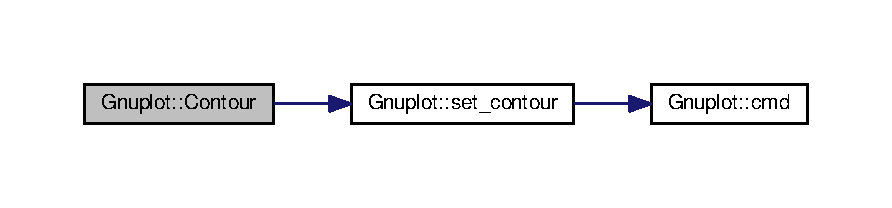
\includegraphics[width=350pt]{classGnuplot_a826a0f860cd984748f8c7ee80228fce7_cgraph}
\end{center}
\end{figure}


\hypertarget{classGnuplot_a42dfb8c9d4636745c7be277ed818e849}{\index{Gnuplot@{Gnuplot}!plot\-\_\-equation@{plot\-\_\-equation}}
\index{plot\-\_\-equation@{plot\-\_\-equation}!Gnuplot@{Gnuplot}}
\subsubsection[{plot\-\_\-equation}]{\setlength{\rightskip}{0pt plus 5cm}{\bf Gnuplot} \& Gnuplot\-::plot\-\_\-equation (
\begin{DoxyParamCaption}
\item[{const std\-::string \&}]{equation, }
\item[{const std\-::string \&}]{title = {\ttfamily \char`\"{}\char`\"{}}}
\end{DoxyParamCaption}
)}}\label{classGnuplot_a42dfb8c9d4636745c7be277ed818e849}


Plota uma equacao fornecida como uma std\-::string y=f(x). Escrever somente a funcao f(x) e nao y= A variavel independente deve ser x Os operadores binarios aceitos sao\-: $\ast$$\ast$ exponenciacao,. 


\begin{DoxyItemize}
\item multiplicacao, / divisao,
\end{DoxyItemize}

adicao,
\begin{DoxyItemize}
\item subtracao, \% modulo Os operadores unarios aceitos sao\-:
\item menos, ! fatorial Funcoes elementares\-: rand(x), abs(x), sgn(x), ceil(x), floor(x), int(x), imag(x), real(x), arg(x), sqrt(x), exp(x), log(x), log10(x), sin(x), cos(x), tan(x), asin(x), acos(x), atan(x), atan2(y,x), sinh(x), cosh(x), tanh(x), asinh(x), acosh(x), atanh(x) Funcoes especiais\-: erf(x), erfc(x), inverf(x), gamma(x), igamma(a,x), lgamma(x), ibeta(p,q,x), besj0(x), besj1(x), besy0(x), besy1(x), lambertw(x) Funcoes estatisticas\-: norm(x), invnorm(x) 
\end{DoxyItemize}

Here is the call graph for this function\-:
\nopagebreak
\begin{figure}[H]
\begin{center}
\leavevmode
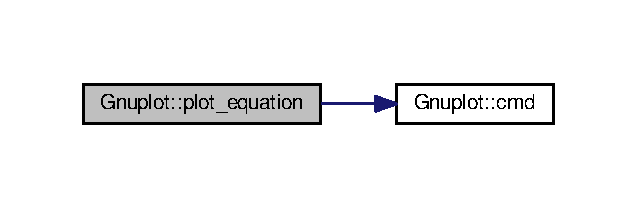
\includegraphics[width=306pt]{classGnuplot_a42dfb8c9d4636745c7be277ed818e849_cgraph}
\end{center}
\end{figure}




Here is the caller graph for this function\-:
\nopagebreak
\begin{figure}[H]
\begin{center}
\leavevmode
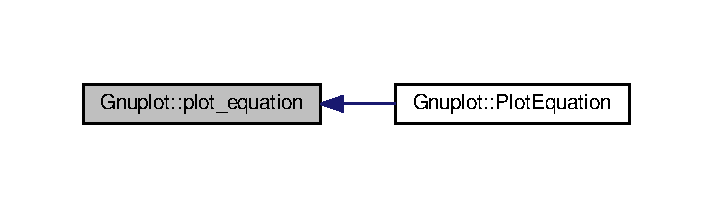
\includegraphics[width=342pt]{classGnuplot_a42dfb8c9d4636745c7be277ed818e849_icgraph}
\end{center}
\end{figure}


\hypertarget{classGnuplot_ab71117b8fa74d53ea20c313717d86b5c}{\index{Gnuplot@{Gnuplot}!plot\-\_\-image@{plot\-\_\-image}}
\index{plot\-\_\-image@{plot\-\_\-image}!Gnuplot@{Gnuplot}}
\subsubsection[{plot\-\_\-image}]{\setlength{\rightskip}{0pt plus 5cm}{\bf Gnuplot} \& Gnuplot\-::plot\-\_\-image (
\begin{DoxyParamCaption}
\item[{const unsigned char $\ast$}]{uc\-Pic\-Buf, }
\item[{const int}]{i\-Width, }
\item[{const int}]{i\-Height, }
\item[{const std\-::string \&}]{title = {\ttfamily \char`\"{}\char`\"{}}}
\end{DoxyParamCaption}
)}}\label{classGnuplot_ab71117b8fa74d53ea20c313717d86b5c}


Plota uma imagem. 


\begin{DoxyItemize}
\item note that this function is not valid for versions of G\-N\-U\-Plot below 4.\-2 
\end{DoxyItemize}

Here is the call graph for this function\-:
\nopagebreak
\begin{figure}[H]
\begin{center}
\leavevmode
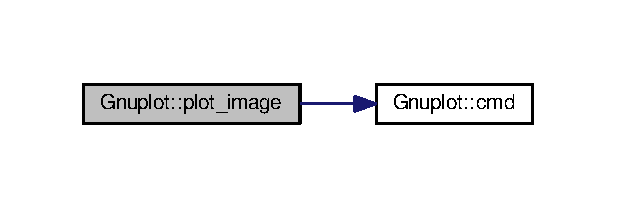
\includegraphics[width=296pt]{classGnuplot_ab71117b8fa74d53ea20c313717d86b5c_cgraph}
\end{center}
\end{figure}




Here is the caller graph for this function\-:
\nopagebreak
\begin{figure}[H]
\begin{center}
\leavevmode
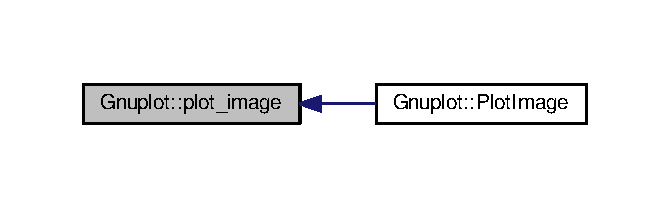
\includegraphics[width=322pt]{classGnuplot_ab71117b8fa74d53ea20c313717d86b5c_icgraph}
\end{center}
\end{figure}


\hypertarget{classGnuplot_af845efc728a90d7e10de764eff0b2423}{\index{Gnuplot@{Gnuplot}!set\-\_\-contour@{set\-\_\-contour}}
\index{set\-\_\-contour@{set\-\_\-contour}!Gnuplot@{Gnuplot}}
\subsubsection[{set\-\_\-contour}]{\setlength{\rightskip}{0pt plus 5cm}{\bf Gnuplot} \& Gnuplot\-::set\-\_\-contour (
\begin{DoxyParamCaption}
\item[{const std\-::string \&}]{position = {\ttfamily \char`\"{}base\char`\"{}}}
\end{DoxyParamCaption}
)}}\label{classGnuplot_af845efc728a90d7e10de764eff0b2423}


Ativa desenho do contorno em superficies (para plotagen 3d). 


\begin{DoxyParams}{Parameters}
{\em base,surface,both.} & \\
\hline
\end{DoxyParams}


Here is the call graph for this function\-:
\nopagebreak
\begin{figure}[H]
\begin{center}
\leavevmode
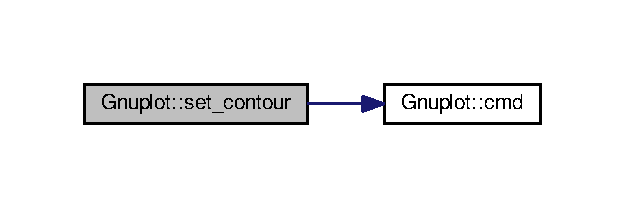
\includegraphics[width=300pt]{classGnuplot_af845efc728a90d7e10de764eff0b2423_cgraph}
\end{center}
\end{figure}




Here is the caller graph for this function\-:
\nopagebreak
\begin{figure}[H]
\begin{center}
\leavevmode
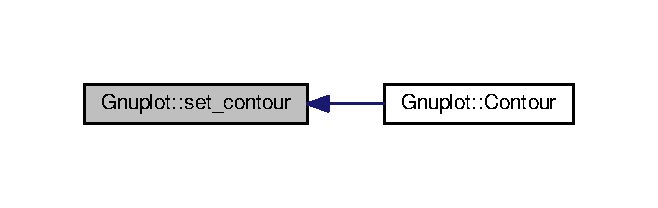
\includegraphics[width=316pt]{classGnuplot_af845efc728a90d7e10de764eff0b2423_icgraph}
\end{center}
\end{figure}


\hypertarget{classGnuplot_a95ec1636a871447dfe99463b769339c7}{\index{Gnuplot@{Gnuplot}!set\-\_\-pointsize@{set\-\_\-pointsize}}
\index{set\-\_\-pointsize@{set\-\_\-pointsize}!Gnuplot@{Gnuplot}}
\subsubsection[{set\-\_\-pointsize}]{\setlength{\rightskip}{0pt plus 5cm}{\bf Gnuplot} \& Gnuplot\-::set\-\_\-pointsize (
\begin{DoxyParamCaption}
\item[{const double}]{pointsize = {\ttfamily 1.0}}
\end{DoxyParamCaption}
)}}\label{classGnuplot_a95ec1636a871447dfe99463b769339c7}


Desativa suavizacao. 

Escala o tamanho do ponto usado na plotagem. 

Here is the call graph for this function\-:
\nopagebreak
\begin{figure}[H]
\begin{center}
\leavevmode
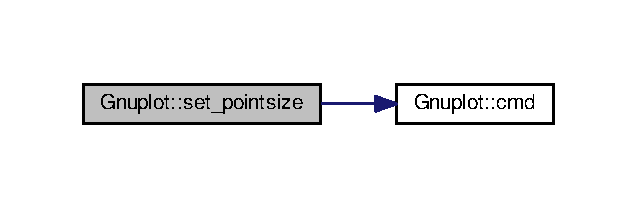
\includegraphics[width=306pt]{classGnuplot_a95ec1636a871447dfe99463b769339c7_cgraph}
\end{center}
\end{figure}




Here is the caller graph for this function\-:
\nopagebreak
\begin{figure}[H]
\begin{center}
\leavevmode
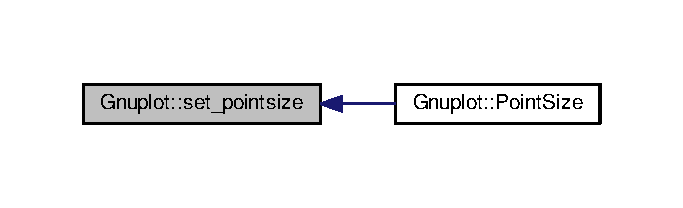
\includegraphics[width=328pt]{classGnuplot_a95ec1636a871447dfe99463b769339c7_icgraph}
\end{center}
\end{figure}




The documentation for this class was generated from the following files\-:\begin{DoxyCompactItemize}
\item 
cgnuplot.\-h\item 
cgnuplot.\-cpp\end{DoxyCompactItemize}

\hypertarget{classGnuplotException}{\section{Gnuplot\-Exception Class Reference}
\label{classGnuplotException}\index{Gnuplot\-Exception@{Gnuplot\-Exception}}
}


Erros em tempo de execucao.  




{\ttfamily \#include $<$cgnuplot.\-h$>$}



Inheritance diagram for Gnuplot\-Exception\-:
\nopagebreak
\begin{figure}[H]
\begin{center}
\leavevmode
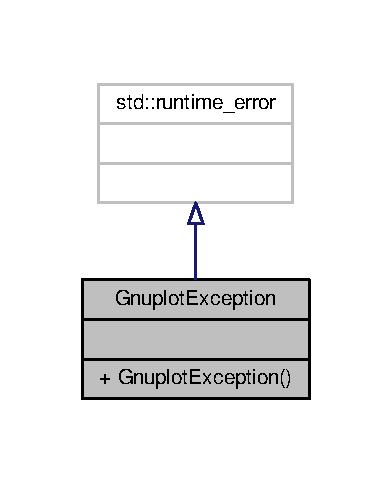
\includegraphics[width=188pt]{classGnuplotException__inherit__graph}
\end{center}
\end{figure}


Collaboration diagram for Gnuplot\-Exception\-:
\nopagebreak
\begin{figure}[H]
\begin{center}
\leavevmode
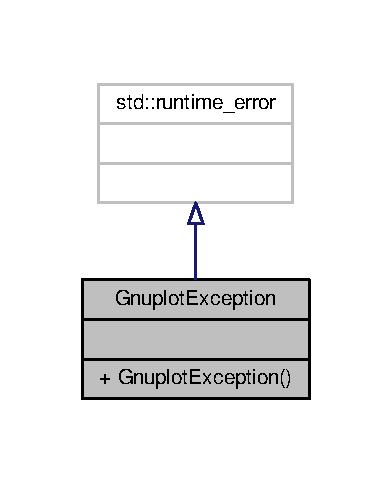
\includegraphics[width=188pt]{classGnuplotException__coll__graph}
\end{center}
\end{figure}
\subsection*{Public Member Functions}
\begin{DoxyCompactItemize}
\item 
\hypertarget{classGnuplotException_a8b324a9ef4d3f75079d41ecd61c62d44}{\hyperlink{classGnuplotException_a8b324a9ef4d3f75079d41ecd61c62d44}{Gnuplot\-Exception} (const std\-::string \&msg)}\label{classGnuplotException_a8b324a9ef4d3f75079d41ecd61c62d44}

\begin{DoxyCompactList}\small\item\em Construtor. \end{DoxyCompactList}\end{DoxyCompactItemize}


\subsection{Detailed Description}
Erros em tempo de execucao. 

The documentation for this class was generated from the following file\-:\begin{DoxyCompactItemize}
\item 
cgnuplot.\-h\end{DoxyCompactItemize}

%--- End generated contents ---

% Index
\newpage
\phantomsection
\addcontentsline{toc}{chapter}{Index}
\printindex

\end{document}
